\documentclass[10pt]{report}
\usepackage[utf8]{inputenc}
\usepackage[top=2cm, bottom=2cm, left=2cm, right=2cm]{geometry}
\usepackage[francais]{babel}
\usepackage{helvet}
\usepackage[T1]{fontenc}
\usepackage{graphicx}
\usepackage{subcaption}
\usepackage{lmodern}
\usepackage{listings}
\usepackage{amsmath} 
\usepackage{algorithm}
\usepackage[noend]{algpseudocode}
\usepackage{wrapfig}
\usepackage[colorlinks=true, linkcolor=black, urlcolor=blue, breaklinks, pagebackref, citebordercolor={0 0 0}, filebordercolor={0 0 0}, linkbordercolor={0 0 0}, pagebordercolor={0 0 0}, runbordercolor={0 0 0}, urlbordercolor={0 0 0}, pdfborder={0 0 0}]{hyperref}  %désactive les cadres autour des liens
\usepackage{etoolbox}
\usepackage{setspace}
\onehalfspacing
\renewcommand{\familydefault}{\sfdefault}

% Supprime l'espace avant l'en-tête des chapitres
\makeatletter
% les chapitres normaux
\patchcmd{\@makechapterhead}{\vspace*{50\p@}}{}{}{}	
% les chapitres étoilés
\patchcmd{\@makeschapterhead}{\vspace*{50\p@}}{}{}{}
\makeatother



\begin{document}

\begin{titlepage}	
	\flushleft
	\begin{figure}[!h]
		
\includegraphics[height=1.8cm]{Reports/figures/logo_insa_cvl.png}
		\hfill
		
\includegraphics[height=3cm]{Reports/figures/logo_biomedia.png}
	\end{figure}
	\centering
	\vspace{2cm}
	{\scshape\Large Stage industriel de 4ème année\par}
	\vspace{1.5cm}
	{\huge\bfseries Développement d'une bibliothèque mathématique performante pour le traitement d'images médicales\par}
	\vspace{2cm}
	{\Large\itshape Élève ingénieur: François PIAT\par}
		\vspace{1cm}
	\begin{figure}[!h]
		\begin{center}
			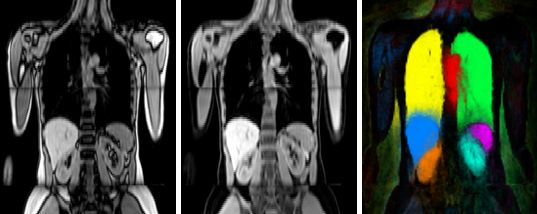
\includegraphics[width=13cm]{Reports/figures/biomedia_image.png}
		\end{center}
	\end{figure}
	\vfill
	\flushleft
	Tuteur INSA: \hfill Tuteurs BioMedIA: \par
	Dr. Julien \textsc{Olivier} \hfill Dr. Ghislain-Anthony \textsc{Vaillant} \\ \hfill Dr. Jonathan \textsc{Passerat-Palmbach}
	\vfill
	% Bottom of the page
	\centering
	{\large Année universitaire 2015 - 2016 \par}
\end{titlepage}

\section*{Remerciements}
En plus de mes 2 tuteurs Dr. Julien OLIVIER et Dr. Ghislain-Anthony VAILLANT, je souhaite remercier Dr. Jonathan PASSERAT-PALMBACH qui a joué un rôle important dans le projet qui incluait les stages de M. Maxime NOEL et moi-même. Il a ainsi su me venir en aide sur le plan technique dès que la situation le permettait.
\newpage
\subsection*{RESUME} 
~\par 
Au sein du laboratoire BioMedIA, situé dans le département informatique de l'Imperial College London, plusieurs projets ont vu le jour depuis la mise en place de UK BioBank, qui sera d'ici quelques années la plus grosse banque de données médicales en Europe. BioMedIA a développé un logiciel, codé en C++, de traitement d'images médicales : le Medical Image Registration Tool-Kit (MIRTK). Ce logiciel pourrait intervenir comme un des outils d'analyse des données de UK BioBank. Cependant, le MIRTK ne possède pas encore les optimisations nécessaires pour s'intégrer dans un projet d'une telle ampleur.\\
Dans ce cadre, ce stage a eu pour but d'améliorer le temps d'exécution du MIRTK sur une machine. La fonction principale du MIRTK est d'effectuer un recalage d'images, c'est-à-dire une "mise en correspondance" de deux images. Le MIRTK traite des images en 3 dimensions, pouvant provenir de plusieurs sources médicales (scanner, scintigraphie, échographie, rayons X ...) au format NIFTI. Ce travail a été réalisé sur le module de calcul mathématique, en y insérant une bibliothèque, appelée ArrayFire, traitant de manière vectorisée des calculs matriciels et offrant aussi la possibilité de rendre le logiciel compatible avec une carte graphique. \\
A la fin des 18 semaines de stage, deux fonctions du logiciel ont principalement été impactées: une fonction de floutage et une fonction de transformation homogène (c'est-à-dire translation et/ou rotation), qui interviennent dans les algorithmes d'un recalage. De plus, les améliorations obtenues ont été soutenues par une analyse de performances du MIRTK.
~\par 
\paragraph*{Mots-clés:}
bibliothèque mathématique, calcul vectorisé, carte graphique, flou, imagerie médicale, performances, recalage, temps d'exécution, traitement d'image, transformation.
~\par \vspace{0.5cm}
\subsection*{ABSTRACT}
~\par
Into the BioMedIA laboratory, located in the cmoputing department of the Imperial College London, some projects has been started since the UK BioBank set up, which will be, within a few years from now, the largest medical data bank in Europe. BioMedIA developped an image proccessing software, coded in C++, named Medical Image Registration Tool-Kit (MIRTK). This sofwtare could be one of the data analysis tools for UK BioBank. However, the MIRTK is not optimized enough yet to be integrated in such a big project.\\
Considering this remit, this internship has been an opportunity to decrease the run time of the MIRTK on one machine. The main function of the MIRTK is to register images, i.e. make the link between two images. The MIRTK processes 3 dimensions images, extracted from several medicale sources (medical scanner, scintigraphy, ultrasound, X-rays...) formatted as NIFTI. This work has been carried out on the numeric computing module, by integrating a library, named ArrayFire, which processes a vectorized matrix computation and adds the option to make the software compatible with a Graphical Processing Unit (GPU).\\
After 18 weeks, two functions have been modified: a blurring function and a homogeneous transformation function (i.e. translation and/or rotation), which are involved in registration algorithms. Finally, the effective improvements have been checked by a performance test of the MIRTK. 	

\paragraph*{Key-words:} blurring, GPU, image processing, mathematics library, medical imaging, performances, registration, run-time, transformation, vectorized computation.

\renewcommand\contentsname{Sommaire}
\tableofcontents

\newpage

\chapter*{Introduction}
\addcontentsline{toc}{chapter}{Introduction}
Dans le cadre de mon stage de quatrième année à l'INSA Centre Val de Loire, j'ai intégré l'équipe du laboratoire BioMedIA, à l'Imperial College London. Ce laboratoire de recherche produit des outils informatiques nécessaires aux chercheurs du milieu médical. Présentant l'occasion de m'intéresser au secteur de la recherche, ce stage m'a semblé approprié pour explorer une filière qui m'était encore inconnue en informatique: le traitement d'image.\\ ~\par  \noindent
Afin de suivre les avancées de la recherche en milieu médical, les outils empruntés à des secteurs transverses tels que l'informatique, l'électronique ou encore la biomécanique doivent constamment respecter la demande de ces chercheurs. L'acquisition de données médicales rassemblant de plus en plus de données visualisables sur ordinateur, elle nécessite des outils de plus en plus rapides et performants en matière de traitement d'images. Outre l'amélioration par ajout de nouvelles fonctionnalités, il est pertinent de fournir aux produits informatiques une maintenance continue. 
\\Dans cette optique, la problématique générale dans laquelle le stage s'installe a été portée sur l'amélioration des performances d'un logiciel de traitement d'images. Afin de satisfaire cette problématique, plusieurs axes ont été développés par le laboratoire BioMedIA, et ont donné lieu à plusieurs sujet de stages. La position de mon sujet vis-à-vis de ce projet a été de réduire le temps d'exécution du logiciel sur une machine par une ré-implémentation de certaines de ses fonctions.  \\ ~\par
\noindent
La première partie du rapport présentera les conditions dans lesquelles le stage s'est déroulé. En plus du lieu de travail, le cadre du projet global sera détaillé.\\
Par la suite, la problématique justifiera le sujet de stage, et le cahier des charges à respecter sera explicité. Une planification des objectifs sera aussi chronologiquement établie.\\
La démarche sera ensuite décrite, avec toutes les notions abordées, les fonctions modifiées, et les algorithmes employés. Toutes les améliorations apportées au logiciel seront soutenues par une série de tests, présentée en fin de rapport.\\
La dernière partie de ce rapport sera dédiée aux perspectives de développement futures du projet, à court et long terme.


\chapter{Environnement de travail} 
	Cette section détaille l'environnement dans lequel s'est déroulé le stage. Le laboratoire sera d'abord présenté puis le cadre du stage sera introduit.
	\section{Le laboratoire}
	
	\subsection{Imperial College London} 
	L’Imperial College London (officiellement The Imperial College of Science, Technology and Medicine) est une université britannique fondée en 1907 par la fusion du City and Guilds College, de la Royal School of Mines et du Royal College of Science (tous fondés entre 1845 et 1878).\\ ~\par
    L'université possède 9 campus au total, tous situés à Londres, et dont la plupart sont implantés dans des sites hospitaliers.  
    Elle possède 5 départements administratifs et 4 branches techniques: ingénierie, sciences naturelles, business, et médecine.	Le campus principal est situé dans le quartier du South Kensington, et regroupe la branche d'ingénierie, de sciences naturelles, d'arts et de business. C'est sur ce campus que le département d'informatique se situe. 
    
	\begin{figure}[h!]
		\begin{center}
			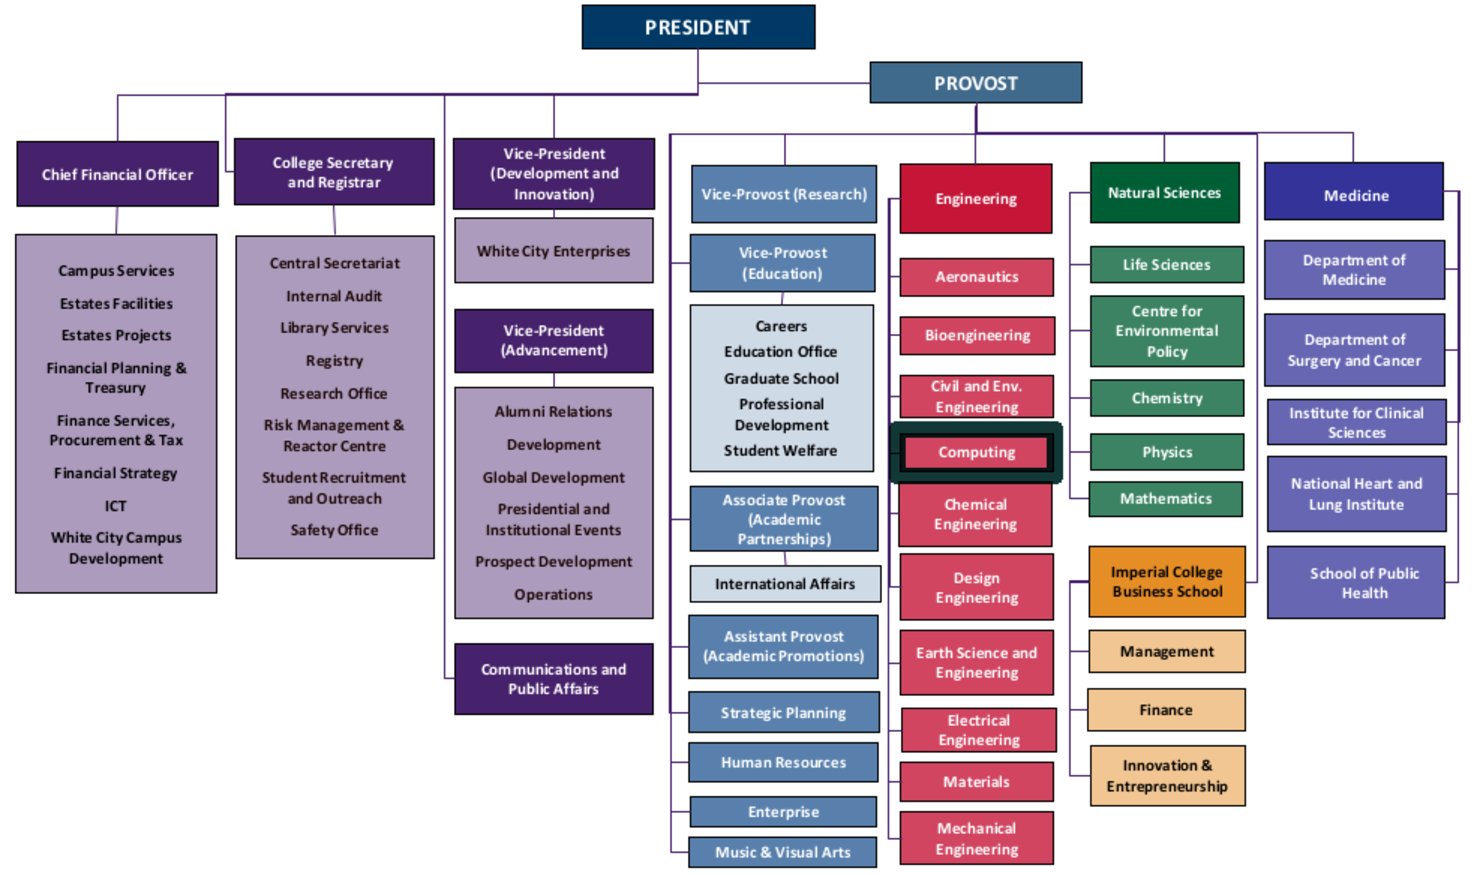
\includegraphics[width=17cm]{Reports/figures/College-Organisation.pdf}
		\end{center}
		\caption[Organigramme de l'Imperial College London]{Organigramme de l'Imperial College London \\ \textit{Le département d'informatique, encadré en noir, se situe dans la branche d'ingénierie (en rouge) de l'université.}}
		\label{Organigramme de l'Imperial College London}
	\end{figure}
	
	\subsection{Le département d'informatique}
	
	Le département d'informatique est divisé en 5 groupes de recherche : 
	\\{$\bullet$}\textit{\textbf{Logic and Artificial Intelligence:}} la recherche en Intelligence Artificielle et Logique englobe des études fondamentales de logique et une variété de disciplines en intelligence artificielle, telles que l'apprentissage automatisé, les flux neurologiques, et la vérification des systèmes autonomes.
	\\{$\bullet$}\textit{\textbf{Distributed Software Engineering:}} la recherche dans le domaine de l'Ingénierie des Logiciels Distribués aborde la conception de systèmes distribués, adaptatifs et fiables.
	\\{$\bullet$}\textit{\textbf{Quantitative Analysis and Decision Science:}} la recherche en Analyse Quantitative et Science de la décision varie de l'optimisation à l'ingénierie de performances, en passant par la des expériences de vérifications quantitatives ou de sécurité.
	\\{$\bullet$}\textit{\textbf{Programming Languages and Systems:}} Systèmes et Langages de Programmation est une section qui combine des travaux théoriques et pratiques en langages et architecture pour obtenir des logiciels rapides, et efficaces.
	\\{$\bullet$}\textit{\textbf{Visual Information Processing:}} la recherche en Traitement d'informations Visualisables couvre une multitude de domaines, incluant la vision numérique, les graphiques, l'apprentissage automatique, et le traitement d'images médicales.
	
	\begin{wrapfigure}[13]{r}{10cm}
		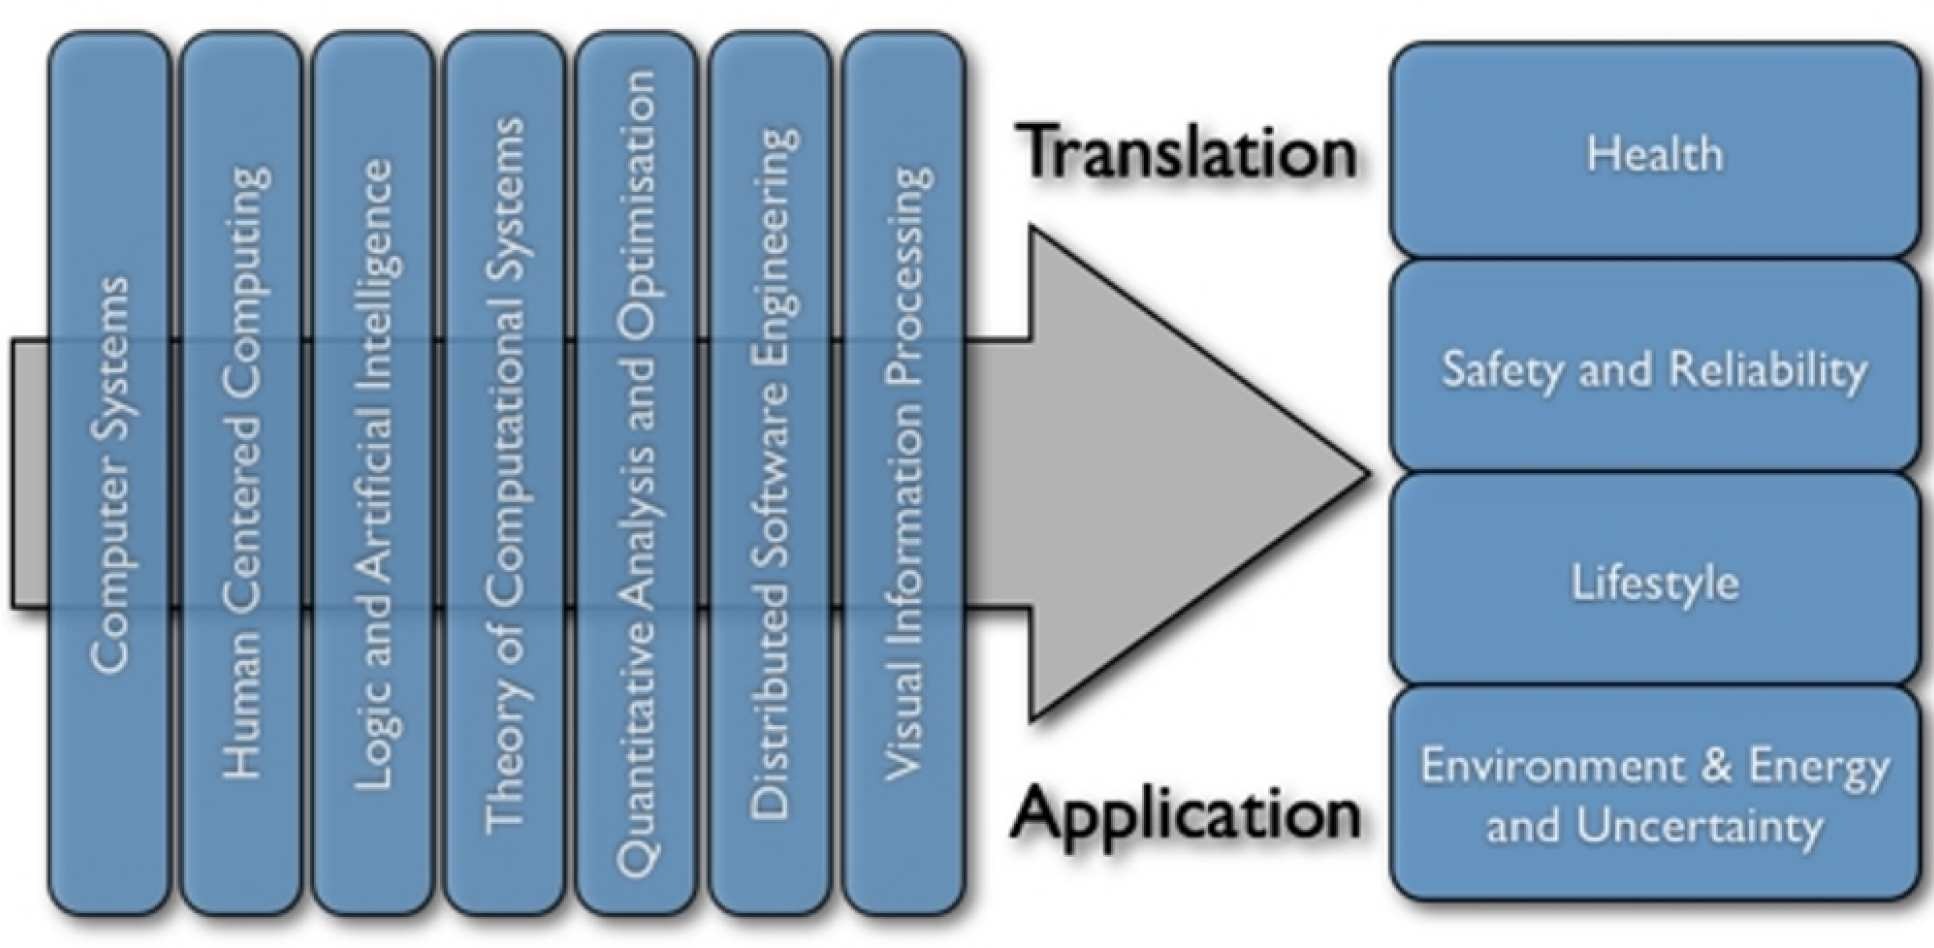
\includegraphics[width=9cm]{Reports/figures/research_strategy.jpg}
		\caption{Stratégie du département de recherche}
		\label{Stratégie du département de recherche}
	\end{wrapfigure}~\par
	
	Les différentes spécialités citées précédemment sont articulées au sein d'un centre de recherche translationnelle, qui se situe à l'intermédiaire entre la recherche fondamentale et la recherche appliquée. La recherche translationnelle s'inspire des travaux de recherche fondamentale et fournit des applications dans les domaines de la santé, de la fiabilité/sécurité, de l'environnement, des modes de vie, de l'énergie et des incertitudes.
	\\
	\\
	\subsection{Le laboratoire BioMedIA}

	La mission du groupe BioMedIA est de développer de nouvelles techniques de
	calcul pour l'analyse d'images biomédicales. Le groupe se concentre sur des
	domaines de recherche de pointe, y compris:\\
	\\{$\bullet$} Le développement d'algorithmes d'acquisition, d'analyse et d'interprétation des images. En particulier dans les domaines du recalage, de la reconstruction,
	du suivi de mouvement, de la segmentation et de la modélisation. \\
	\\{$\bullet$} L'apprentissage machine pour l'extraction d'information clinique à partir
	d'images médicales. Les applications incluent le diagnostic assisté par
	ordinateur, la planification automatisée de traitement médical, ou encore la thérapie et les interventions guidées par ordinateur. \\
	\\Le laboratoire s'intéresse particulièrement à l'imagerie et les technologies de
	traitement informatique qui permet de mieux comprendre le
	développement du cerveau humain, l’évolution des maladies mentales et le
	diagnostic des patients atteints de maladie cardiovasculaire.
	
	\section{Cadre du projet} 
	\subsection{Medical Image Registration Toolkit (MIRTK)}
	Le Medical Image Registration Tool-Kit (abrégé MIRTK) est un logiciel open-source de traitement d'images médicales codé en C++ et utilisé par des chercheurs dans le milieu médical. Il propose différents modules qui sont spécialisés pour le recalage d'images. Le MIRTK prend en charge les formats d'image NIFTI, composé d'une entête fixe contenant des informations sur l'encodage, la géométrie et la localisation de l'image, suivie d'un corps contenant la valeur des différents voxels.   
	L'utilisation du MIRTK se concentre autour d'une interface en lignes de commandes, incluant le nom de la fonction, les paramètres et les arguments nécessaires, et propres à chacune des fonctions. Par exemple, la ligne de commande suivante permet de rogner une image :
	
	\begin{lstlisting}
mirtk extract-image-region input.nii.gz output.nii.gz -Ry1 100 -Ry2 200
	\end{lstlisting}
	
	\noindent Sur cette ligne de commande:\\
	\t{$\bullet$} \textbf{"mirtk"} indique que la commande à exécuter est une commande du MIRTK.\\
	\t{$\bullet$} \textbf{"extract-image-region"} est la commande désirée. Celle-ci effectue un rognage.\\
	\t{$\bullet$} \textbf{"input.nii.gz"} indique l'emplacement et le nom de l'image d'entrée, idem pour la sortie avec \textbf{"output.nii.gz"}. Ces fichiers sont au format NIFTI (ici compressées).\\
	\t{$\bullet$} \textbf{"-Ry1 100 -Ry2 200"} permet de spécifier la région sur laquelle le rognage est effectué. Ici, dans le cadre d'une étude de la section abdominale par exemple, la hauteur de l'image est réduite à la zone d'étude. 
	\\L'action de cette ligne de commande est visualisable sur la Figure \ref{Effet de la fonction "extract-image-region"}.
	
	\begin{figure}[h!]
		\centering
		\begin{subfigure}{.5\textwidth}
			\centering
			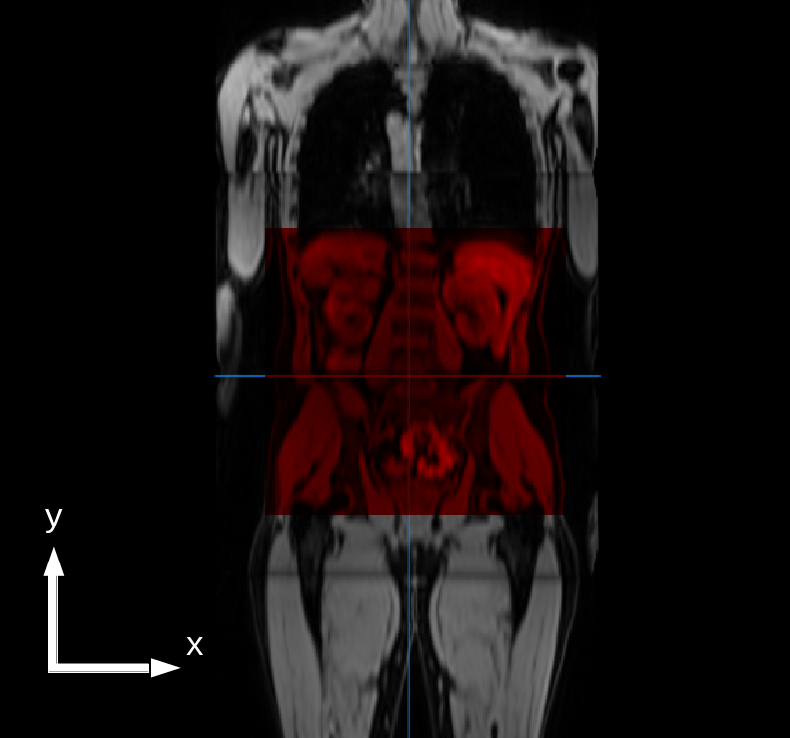
\includegraphics[width=4cm]{Reports/figures/mirtkextractregion1dbis.png}
			\caption{Image d'entrée}
			\label{Image d'entrée}
		\end{subfigure}%
		\begin{subfigure}{.5\textwidth}
			\centering
			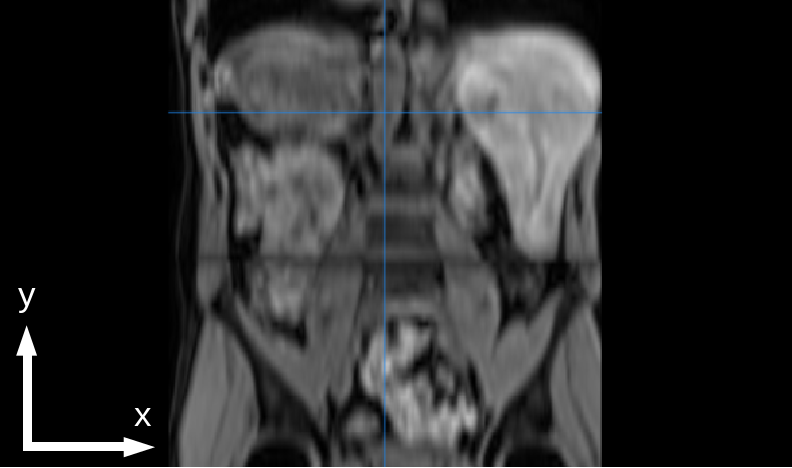
\includegraphics[width=6cm]{Reports/figures/mirtkextractregion21d.png}
			\caption{Image de sortie}
			\label{Image de sortie}
		\end{subfigure}
		\caption{Effet de la fonction "extract-image-region"}.
		\label{Effet de la fonction "extract-image-region"}
	\end{figure}	
	\vspace{-0.5cm}
	Le dossier \textit{Applications} du MIRTK regroupe les fichiers correspondants aux commandes exécutables. Ils font appel à certaines dépendances, qui sont réparties en 7 modules : \textit{Common, Image, I/O, Numerics, PointSet, Registration} et \textit{Transformation}. 
	 Le recalage d'image (Registration) est l'une de ses principales fonctions.
	
	 \subsection{UK BioBank}

	 \textit{UK BioBank} est une association fournissant la banque de données médicales la plus importante du Royaume-Uni. Elle a pour but d'améliorer la prévention, le diagnostic et le traitement d'un large éventail de maladies graves, y compris le cancer, les maladies cardiaques, les accidents vasculaires cérébraux, le diabète, l'arthrite, l'ostéoporose, les affections oculaires, la dépression et les formes de démence. 500.000 personnes âgées de 40 à 69 ans ont été recrutées sur la période 2006-2010 à l'échelle nationale pour prendre part à ce projet. Ils ont accepté de donner leur sang, leur urine et des échantillons de salive pour une analyse future, ainsi que des informations détaillées sur eux-mêmes et sur leur santé. D'ici quelques années, ce processus permettra aux chercheurs d'identifier les critères qui influent le développement de certaines maladies.
	 	 
\chapter{Objectifs et cahier des charges}
	Ce chapitre détaille la motivation du stage, le cahier des charges et la planification des différentes étapes du projet.
	\section{Problématique} 
	Jusqu'ici, le MIRTK a été utilisé pour des études de tailles modestes, dont la validation s'effectue sur une dizaine voire une centaine de patients. Pour cet ordre de grandeur, les performances actuelles du MIRTK sont suffisantes. Cependant avec UK BioBank, cette ordre de grandeur va être multiplié par 10, 100, voire 1000 et le moindre gain de performances, à l'échelle du MIRTK, impactera le temps d'exécution globale sur la base de données UK BioBank.\\ ~\par
	
	Afin d'accélérer leur temps de traitement, les calculs du MIRTK peuvent être effectués sur différents environnement d'exécution*:
	\\{$\bullet$}\textbf{ sur une machine en local}, 
	qui distribuera les tâches sur différents cœurs d'exécution et profitera des divers niveaux de cache du processeur pour accélérer les accès mémoire. Les meilleurs processeurs à l'heure actuelle possède quelques dizaines cœurs et jusqu'à 20 MB de mémoire cache.
	\\{$\bullet$}\textbf{une solution d'ordonnancement de tâches informatiques}, tel que SLURM \textit{(Simple Linux Utility for Resource Management)}, qui permettrait de déployer et gérer des tâches simultanément sur plusieurs machines. 
	\\{$\bullet$}\textbf{une grille de calculs}, qui est une infrastructure virtuelle fournissant ensemble de ressources informatiques (dont des environnements d'exécution*) et mise à disposition d'entreprises et/ou de chercheurs. \newline
	Par exemple, les chercheurs du laboratoire BioMedIA utilisent les grilles suivantes : \\
	\t - La grille de l'Imperial College, qui s'étend à tout le réseau de machines de l'université, mais qui est un service payant. Cette grille met au total 5300 cœurs d'exécution à disposition.\\
	\t - La grille européenne, financée par l'Union Européenne et conduite par le CERN, qui met à disposition des services informatiques aux organismes européens de recherche. Ces services comprennent des environnements d'exécution* et plus de 500 PétaBytes de stockage de données (1 Pétabyte = 10\up{15} bytes). Concernant les environnements d'exécution*, la grille fournit au total plus de 650 000 cœurs.
	\\{$\bullet$}\textbf{ dans le "cloud"}, c'est-à-dire un service proposé par des entreprises telles que Microsoft ou Amazon, qui permet la location d'un serveur distant, moyennant un certain coût. \\ ~\par
	En revanche, ces différents services possèdent chacun certaines contraintes. L'exécution sur un réseau local, une grille de calculs fournie par l'université ou un cloud implique un coût qui peut rapidement devenir prohibitif. Un slurm ou une grille de calculs mutualisée utilisent les performances d'autres machines, qui, elles-même peuvent éventuellement être déjà occupées par l'exécution d'autres tâches. La réduction du temps d'exécution du MIRTK représenterait un coût moindre dans un cas, sinon un impact plus faible sur les ressources mutualisées.\\ 
	Plusieurs directions sont possibles pour optimiser la durée de ces réquisitions. L'optimisation pourra intervenir au niveau de l'exécution multi-machines: c'est sur cet aspect qu'a travaillé Mr. Maxime Noël, dans le cadre de son stage intitulé:"Interfaçage de fonctions de traitement d'images médicales à une bibliothèque Python et intégration dans un outil de workflow".\\
	\vspace{-0.7cm}

	Une autre possibilité d'optimisation sera la réduction du temps d'exécution sur une machine. Pour cela, le MIRTK utilise une technique d'optimisation appelée "la parallélisation" d'un code. 
	A l'inverse de l'exécution séquentielle, la parallélisation consiste à mettre en œuvre des architectures d'électronique numérique permettant de traiter des informations de manière simultanée, ainsi que les algorithmes spécialisés pour celles-ci. Ces techniques ont pour but de réaliser le plus grand nombre d'opérations en un temps le plus court possible.
	Un algorithme adapté pour la parallélisation partage l'exécution globale d'un programme en plusieurs "blocks" d'exécution, chacun correspondant à un groupe d'instructions. La figure \ref{Fonctionnement d'une boucle en parallèle} représente ce principe avec des blocks de 2 itérations.
	\begin{figure}[h!]
		\begin{center}
			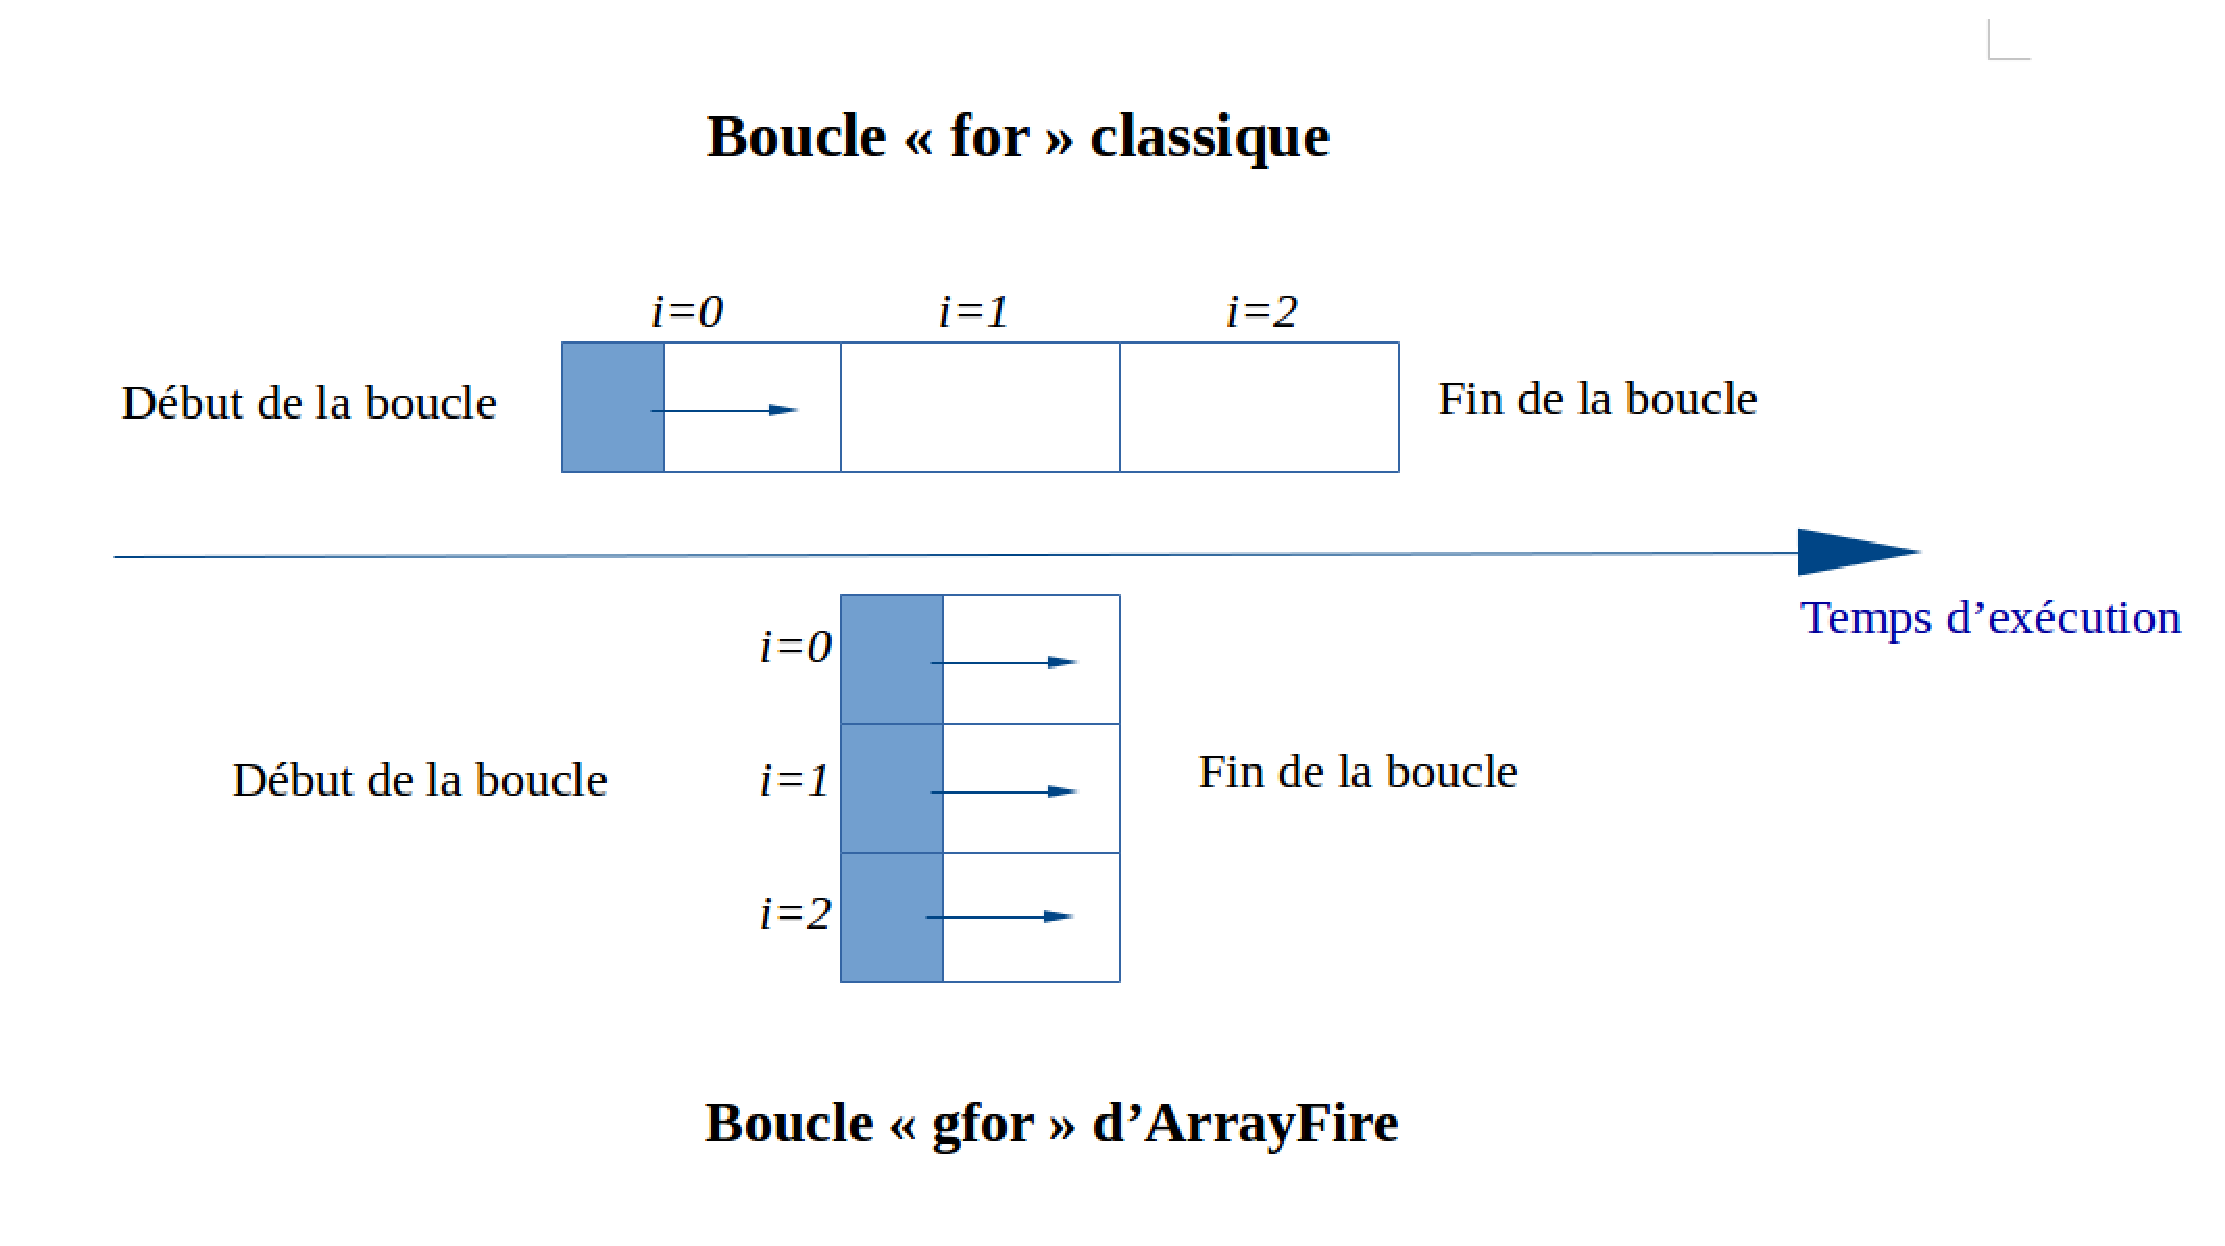
\includegraphics[width=14cm]{Reports/figures/gfor.eps}	
		\end{center}
		\caption{Fonctionnement d'une boucle en parallèle}
		\label{Fonctionnement d'une boucle en parallèle}
	\end{figure}
	~\par
	Le calcul par le GPU*, ou le GPGPU (General-Purpose computing on Graphics Processing Units) permet de paralléliser les tâches et d'offrir un maximum de performances dans de nombreuses applications : le GPU accélère les portions de code les plus lourdes en ressources de calcul, le reste de l'application étant géré par le CPU*. Les applications des utilisateurs s'exécutent ainsi bien plus rapidement.\\
	Pour comprendre les différences fondamentales entre un CPU et un GPU, il suffit de comparer leur manière de traiter chaque opération. Les CPU incluent un nombre restreint de cœurs optimisés pour l'exécution de noyaux complexes, alors que les GPU intègrent des milliers de cœurs conçus pour traiter efficacement de nombreux noyaux simples simultanément.\\
	Les GPU incluent des milliers de cœurs pour traiter efficacement des tâches parallèles. \\ 
	 
	A l'heure actuelle, le MIRTK bénéficie seulement du multi-threading* pour l'instant, et nécessite une amélioration sur le plan de ses performances sur plusieurs cœurs. De plus,  le MIRTK n'est pas encore capable d'utiliser d'accélérations matérielles telles que l'utilisation de GPU.
	\newpage
	\section{Cahier des charges}
	La réduction du temps d'exécution est l'axe principal de développement du stage. Pour cela, l'amélioration devra se concentrer sur les fonctions élementaires du MIRTK les plus consommatrices en ressource de calcul. Dans le cadre du stage, l'intervention se fera au niveau de son implémentation concrète sur CPU et GPU, appelée "backend" par la suite.\\ ~\par
	
	\noindent Dans le cadre du stage, les besoins suivants ont été définis : \\
	\\{$\bullet$} Rendre l'exécution du MIRTK possible sur GPU. A l'heure actuelle, le MIRTK utilisent uniquement les quelques cœurs d'un processeur et ne tire pas encore l'avantage des capacités d'un GPU.\\
	\\{$\bullet$} Conserver une exécution transparente du code, en n'altérant ni les lignes de commandes utilisées, ni le résultat attendu.  \\
	\\{$\bullet$} Dans la mesure du possible, un réusinage* du code devra être opéré. Suite à la modification du code du MIRTK, ainsi qu'à l'ajout probable certaines fonctionnalités, il est possible que des doublons subsistent, et que la lisibilité de certaines parties du code peut s'améliorer.	
	\section{Planification}
	\subsection{Objectifs} 
	Les objectifs de stage sont définis de la manière chronologique suivante:
	~\par~\par 
	1) \textbf{Étude du MIRTK et de ses dépendances} \\
	Cette étape préliminaire a pour but de comprendre le fonctionnement global du MIRTK et de se familiariser avec son code source. 
	~\par~\par 
	2)\textbf{Analyse de l'interface d'ArrayFire} \\
	Dans le même temps, une analyse de l'interface d'ArrayFire, une bibliothèque mathématique optimisée, et des différentes fonctions proposées par la bibliothèque sera entreprise. Cette étude corrélera les besoins du MIRTK et les solutions proposées par ArrayFire.
	~\par~\par 
	\t 3) \textbf{Intégration de ArrayFire dans le MIRTK} \\
	L'étape fondamentale du stage sera la ré-implémentation de différentes fonctions du MIRTK en utilisant ArrayFire.
	~\par~\par 
	\t 4) \textbf{Analyse des performances} \\
	Un profilage du MIRTK sera effectuée avant et après la modification du code source. Cette étape permettra d'abord de définir les fonctions sur lesquelles il faut agir en priorité, puis de se rendre compte des améliorations apportées lors du stage.
\newpage

\chapter{Réalisation du stage} \vspace{-0.5cm}
Cette partie du rapport présente la bibliothèque ArrayFire, ainsi que son intégration dans le MIRTK.
	\section{Introduction à ArrayFire}
	ArrayFire est une bibliothèque logicielle open-source, proposant une grande variété de fonctions mathématiques optimisées. Elle propose aussi plusieurs fonctionnalités de manipulations de backends afin d'exécuter le même code sur différentes configurations matérielles.
	\subsection{Les fonctions mathématiques}
	L'interface d'ArrayFire repose sur la manipulation d'un type générique de tableau nommé \textit{af::array}. Celui-ci peut contenir tout type de valeurs numériques (entier, flottant ou complexe) et peut être utiliser pour représenter des structures de données allant jusqu'à 4 dimensions, comme des vecteurs, matrices, images, volumes, ou série de volumes. Ce type présente plusieurs constructeurs, et ceux-ci peuvent faire appel à une variable appelée \textit{af::dim4} qui est un ensemble de 4 entiers définissant la taille du tableau sur chacune de ses dimensions.\\ ~\par 
	
	\noindent Autour de ce type s'articulent deux types de fonctions: ~\par 
	- Des fonctions mathématiques basiques qui traitent d'algèbre linéaire, telles que des factorisations, décompositions ou opérations de matrices. Jointes à un jeu de fonctions de manipulations de matrices, cet ensemble constitue un noyau de fonctionnalités mathématiques complet. Dans le cas où ArrayFire ne couvre pas une fonctionnalité particulière, il est possible de l'étendre grâce à ces quelques fonctionnalités de base. Pour des fonctionnalités plus complexes, ArrayFire met à disposition un outil appelé \textit{"GFOR"}, qui représente l'équivalent d'une boucle \textit{"FOR"} classique vectorisée. \\~\par 
	- Des fonctions spécifiques a certains domaines scientifiques, comme le traitement de signal, d'images ou encore les statistiques. La vectorisation de certaines de ces fonctions peut, grâce à un paramètre supplémentaire, être explicitement activée ou désactivée. Dans le cadre du stage, les fonctions de traitement d'images se sont révélées être insuffisantes car uniquement applicables sur des images en 2 dimensions, tandis que le MIRTK traite aussi des images en 3 et 4 dimensions. Il sera en revanche possible de s'inspirer de leur implémentation.
	\subsection{La gestion des backends}
	
	ArrayFire dispose aussi d'un ensemble de modules permettant de manipuler des backends. \\ ~\par
	
	Tout d'abord, l'interface d'ArrayFire est commune à tous les backends, ce qui offre la transparence d'exécution. Le code client cible un backend unifié lors de la compilation, mais on peut définir un backend spécifique concrètement pour une exécution.\\ ~\par

	De plus, un module de bascule dynamique entre plusieurs backends est présent dans la bibliothèque ArrayFire. Grâce à cette fonction, il sera possible d'adapter l'exécution du code entre CPU et GPU. Pour exécuter des fonctions de conversion ou de déclaration en mémoire par exemple, la meilleure solution sera d'utiliser le backend du processeur car celui-ci sera plus adapté pour ce genre de tâches qu'une carte graphique. Avant l'application d'un filtre, on pourra donc, grâce à cette fonctionnalité, basculer l'exécution sur la carte graphique, et ce, de manière transparente.\\
	
	Une autre fonctionnalité permet aussi de détecter les informations matérielles de la machine, en listant les caractéristiques des cartes graphiques et du processeur de la machine sur laquelle l'exécution est lancée. Ce module permet de se rendre compte des performances des différentes entités d'exécution sur la machine et ainsi orienter convenablement l'exécution de chaque fonction.
	
	
	\section{Intégration de ArrayFire dans le MIRTK}
	\subsection{Filtres concernés}
	La fonctionnalité majeure du MIRTK est le recalage d'images médicales. Le recalage est une technique qui consiste en la « mise en correspondance d'images », ceci afin de pouvoir comparer ou combiner leurs informations respectives. Cette mise en correspondance se fait par le recherche d'une transformation géométrique permettant de passer d'une image à une autre. C'est une optimisation, ce qui implique que les différentes étapes nécessaires au calcul de la fonction de coup (ici la similarité) doivent être accélérées.\\
	Le module de recalage du MIRTK utilise notamment des itérations successives de floutages et de transformations. Pour cette raison, ces deux fonctions du MIRTK ont été traitées: \textit{smooth-image} et \textit{transform-image}.
	\paragraph{Algorithme de "smooth-image"}
~\par
	L'algorithme de floutage d'une image est, dans le MIRTK, traité comme une convolution d'un filtre gaussien et les valeurs numériques de chaque voxel* de l'image. Ce procédé est illustré en figure \ref{Principe d'une matrice de convolution pour un filtre}.
	\begin{figure}[h!]
		\begin{center}
			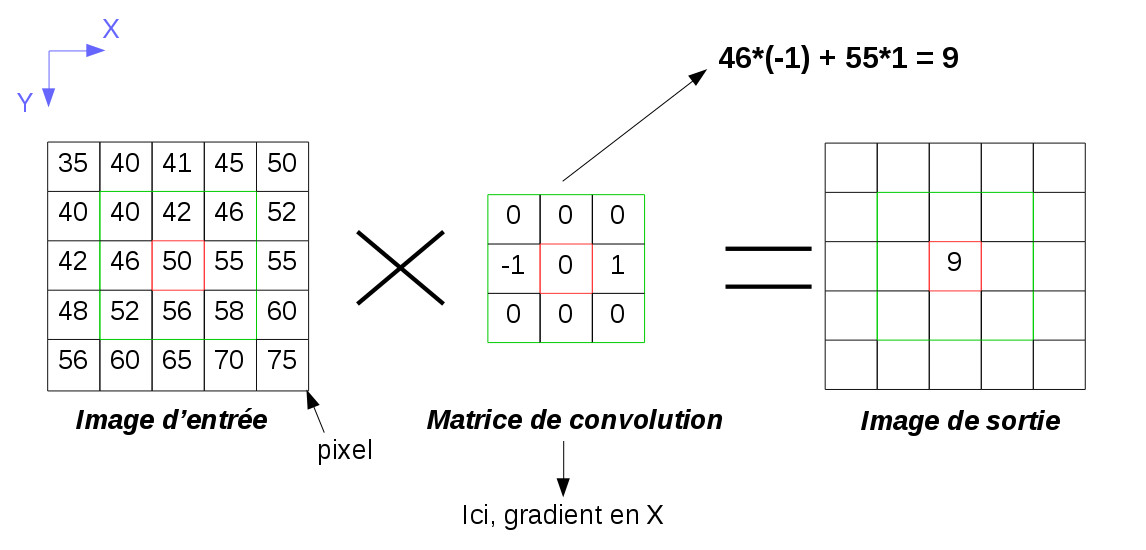
\includegraphics[width=12cm]{convolve.jpg}
		\end{center}
		\caption{Principe d'une matrice de convolution pour un filtre}
		\label{Principe d'une matrice de convolution pour un filtre}
	\end{figure} ~\par
	Sur la figure \ref{Principe d'une matrice de convolution pour un filtre} est traduite un gradient de l'image sur l'axe horizontal. Pour effectuer un floutage de l'image, la méthode précédente reste la même, mais avec une matrice de convolution traduisant un filtre gaussien :
	\begin{figure}[h!]
		\begin{center}
			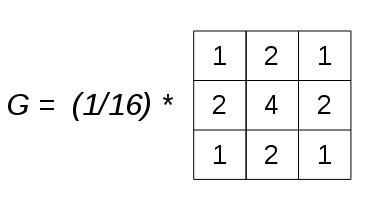
\includegraphics[width=8cm]{matrix_gaussian.jpg}
		\end{center}
		\caption{Matrice de convolution gaussienne}
		\label{Matrice de convolution gaussienne}
	\end{figure} ~\par
	Le MIRTK utilise, à l'heure actuelle, une boucle itérant ce calcul sur chaque pixel de l'image de manière parallélisée, mais le temps d'exécution de la boucle en elle même peut être relativement longue, en fonction de la taille de l'image traitée. 
	Puisqu'une convolution est un produit matriciel, qui peut d'ailleurs être séparable selon les dimensions, la vectorisation est possible et permettrai de palier à ce défaut d'optimisation. C'est ce que fait la fonction \textbf{\textit{af::convolve1(af::array, af::array)}} dans ArrayFire.\\
	Si la convolution s'effectue sur les 3 dimensions, la fonction est exécutée en 3 temps (un pour chaque dimension): la convolution s'exécute entre un filtre gaussien et les valeurs de la première dimension de l'image à chaque itération afin de rendre le floutage séparable. Pour respecter une intégrité du floutage, le contenu de l'image est réarrangé avec la fonction \textbf{\textit{af::reorder(af::array, int, int, int)}} en amenant, pour chaque itération, les valeurs de la dimension à flouter à la place de la première dimension.\\ 
	Contrairement au MIRTK qui itère cette convolution sur chaque pixel de l'image, ArrayFire présente une fonction convoluant directement l'image avec le filtre de manière vectorisée.\\
	Cet algorithme de floutage est détaillé en annexe 2 en langage Python.
	\paragraph{Algorithme de "transform-image"} ~\par
	La transformation d'image a pour but de bouger la position de chacun des voxels de l'image d'entrée, en fonction des paramètres indiqués par dans un fichier décrivant la transformation voulue.\\
	Le MIRTK est apte à traiter des transformations homogènes et non-homogènes. Une transformation homogène applique la même transformation à tous les voxels de l'image, alors qu'une transformation non-homogène est dépendante des coordonnées de chaque voxel.  \\
	Ci-dessous est décrit le procédé de transformation homogène :
	\begin{figure}[h!]
		\begin{center}
			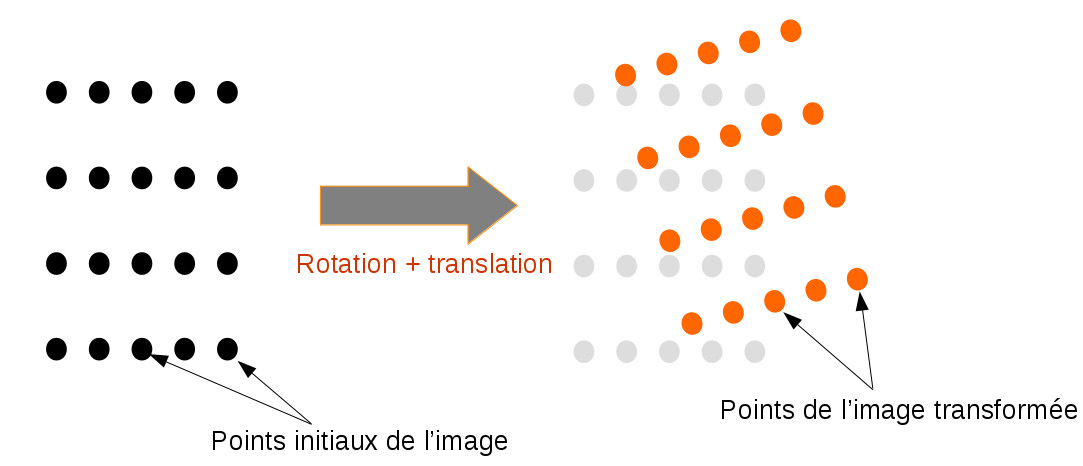
\includegraphics[width=14cm]{transform_trans_rot.jpg}
		\end{center}
		\caption{Principe d'une transformation d'image homogène}
		\label{Principe d'une transformation d'image homogène}
	\end{figure} ~\par
	
	Après la récupération du fichier de transformation, et l'acquisition des points transformés, l'étape suivante est le calcul des distances entre les points transformés et leurs voxels voisins. Les valeurs de ces distances seront nécessaires pour la dernière étape de la transformation: l'interpolation.
	
	\begin{figure}[h!]
		\begin{center}
			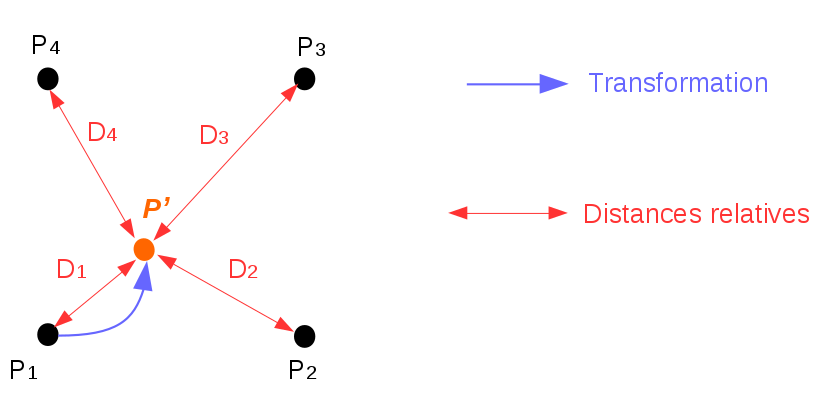
\includegraphics[width=12cm]{transform_image.png}	
		\end{center}
		\caption{Calcul des distances entre les points transformés et les voxels voisins}
		\label{Calcul des distances entre les points transformés et les voxels voisins}
	\end{figure}
	~\par 
	L'interpolation de chaque voxel de l'image de sortie est la dernière étape du procédé de calcul des points transformés, qui peut être réalisé par plusieurs méthodes :\\
	- L'interpolation \textit{Nearest Neighbour}, abrégée NN, qui associe au point transformé son voxel voisin le plus proche. Ci-dessous est détaillé ce type d'interpolation sur l'exemple de la transformation du point P1 en figure \ref{Calcul des distances entre les points transformés et les voxels voisins}.\\
	\begin{figure}[h!]
		\begin{center}
			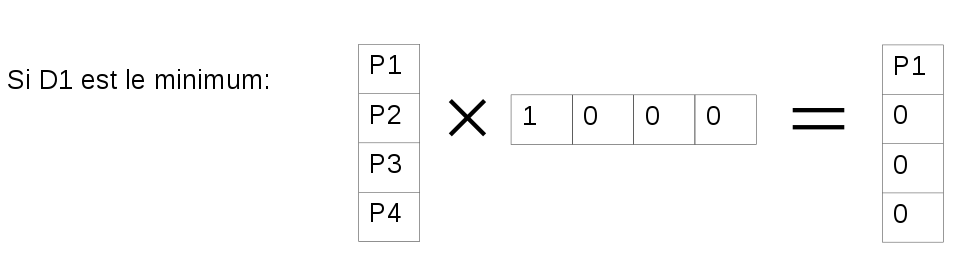
\includegraphics[width=12cm]{calcul_interp_nn.png}	
		\end{center}
		\caption{Interprétation de l'interpolation NN sous forme matricielle}
		\label{Interprétation de l'interpolation NN sous forme matricielle}
	\end{figure}
	~\par 
	- L'interpolation linéaire, qui fait une moyenne pondérée entre les valeurs des voxels voisins, en prenant en poids les distances proportionnelles D1, D2, D3, et D4. L'interprétation matricielle de cette interpolation est la suivante :
	\begin{figure}[h!]
		\begin{center}
			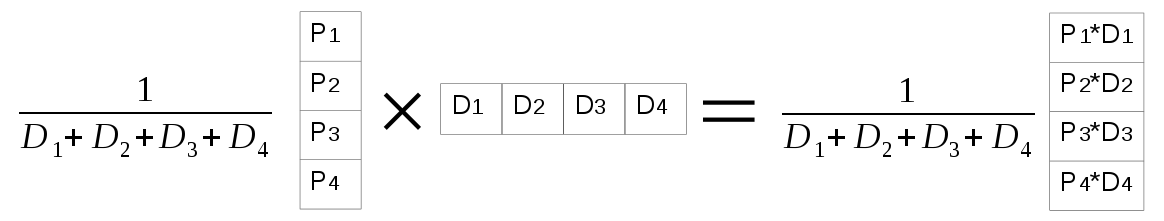
\includegraphics[width=16cm]{calcul_interp_lineaire.png}	
		\end{center}
		\caption{Interprétation de l'interpolation linéaire sous forme matricielle}
		\label{Interprétation de l'interpolation linéaire sous forme matricielle}
	\end{figure}
	~\par 

	

	\section{Évaluation des performances}
	\vspace{0.7cm}
		\subsection{Profilage}
Un profilage est une étude de comportement d'un programme lors de son exécution. Cette étape est un relevé de performances du MIRTK, et, de même que toutes les démarches utilisées dans la partie "Evaluation de performances", ne modifie aucunement le code source du MIRTK. 

\subsubsection{a) Configuration}
\vspace{0.7cm}
	\paragraph{Choix du profileur}~\par

Avant d'effectuer un profilage, il a en premier lieu été nécessaire de choisir le bon outil de profilage. Pour le choisir, ont été définis deux principaux critères:\\
{$\bullet$} Le genre d'informations relevées : dans le cadre du MIRTK il était suffisant de se restreindre au temps d'exécution. En revanche, il était nécessaire d'avoir une fonctionnalité analysant (ou permettant au moins de visualiser) l'exécution parallèle du code. \\
{$\bullet$} L'accès gratuit au programme de profilage, puisqu'il ne sera pas utilisé à long terme.\\
Avec mes tuteurs, nous avons choisi d'utiliser le module \textit{Callgrind} de la suite d'outils \textit{Valgrind}, qui répond à aux critères précédents.
 \paragraph{Présentation de Valgrind et Callgrind}~\par
 La suite d'outils Valgrind présente des modules de débogage, de profilage, et d'analyses de mémoire pour tous types de programmes informatiques. \\
 Le module CallGrind a principalement été utilisé afin de compter le nombre d'appels pour toutes les routines d'un programme durant son exécution, ainsi que le temps passé dans la routine. L'utilisation de Callgrind était essentiellement en ligne de commande, 
 de la manière suivante:
 	\begin{lstlisting}
 	valgrind --tools=callgrind [options] [commande]
 	\end{lstlisting}
 Cette méthode ajoute donc un préfixe à la commande voulue, par exemple le floutage d'une image avec le MIRTK, accompagné de un ou plusieurs options si nécessaires. Dans le cadre du profilage du MIRTK, 3 options ont été régulièrement utilisées: \\
 - \textit{separate-threads}: impose l'analyse indépendante de chaque thread* lors de l'exécution.\\
 - \textit{cache-sim}: simule l'interaction du programme avec la hiérarchie des caches. Cette commande fait appel à l'outil \textit{CacheGrind}.\\
 - \textit{callgrind-out-file}: définit le nom du fichier de profilage généré.\\ ~\par
  \newpage
 Par ailleurs, pour mettre en forme les résultats obtenus par callgrind, le module KCacheGrind a permis de visualiser les fichiers de profilage par l'intermédiaire de l'interface suivante:\\
\begin{figure}[h!]
	\begin{center}
		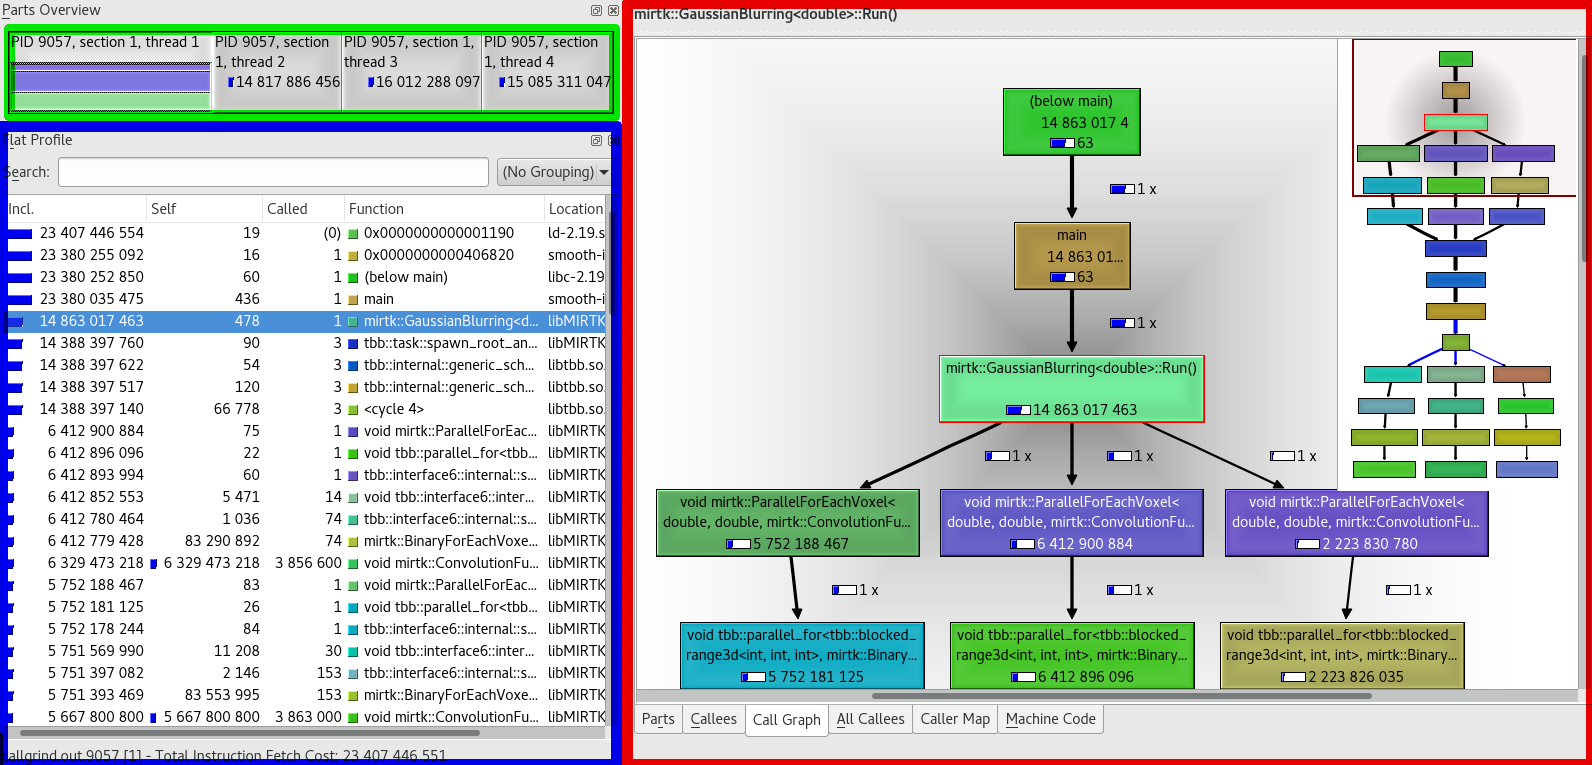
\includegraphics[width=18cm]{Reports/figures/UIkcachegrind.png}	
	\end{center}
	\caption{Interface graphique de KCacheGrind}
	\label{Interface graphique de KCacheGrind}
\end{figure}\\
Cette interface est découpée en 3 secteurs, visibles sur la figure \ref{Interface graphique de KCacheGrind} : \\
- Le cadre vert indique les différents threads d'exécution du programme. Lorsqu'un programme est séquentiel, il n'y a qu'un seul rectangle.\\
- le cadre bleu répertorie toutes les fonctions et du thread sélectionné et les ressources associées à chacune d'elles.\\
- le cadre rouge indique les interdépendances des fonctions du programme. Elles sont ici représentées sous forme de graphe.\\ 

\paragraph{Caractéristiques de la machine utilisées pour le profilage}  ~\par 
Les caractéristiques de la machine ayant déroulé les tests sont les suivantes :\\
 \textbf{GPU:} Tesla K40c / 2880 cœurs, 6GHz, 12 GB de RAM\\
 \textbf{CPU:} Intel(R) Xeon(R) CPU E5-2630 v2 @ / 2.60GHz, 6 cœurs, 15MB de mémoire cache.
\newpage
\subsubsection{b) Résultats}
Le profilage a été exécuté sur l'ensemble du MIRTK, mais les résultats des fonctions de transformation (transform-image) et celles de floutage (smooth-image) sont les plus pertinents. \\
Ces résultats ont été récoltés avec l'exécution des programmes sur la même image en entrée. Cependant, transform-image possède différents moyens d'interpoler les voxels de l'image de sortie, comme expliqué en partie 3.2.1. Il a donc été nécessaire de relever les performances de chaque interpolation: NN, linéaire, sinus cardinal, gaussienne, et B-spline. Une parallélisation du code était présente avant le stage, via la bibliothèque \textit{Threading Building Blocks} (abrégé TBB), et est comparée ci-dessous avec une exécution séquentielle de chaque fonction:
\begin{figure}[h!]
	\centering
	\begin{subfigure}{.5\textwidth}
		\centering
		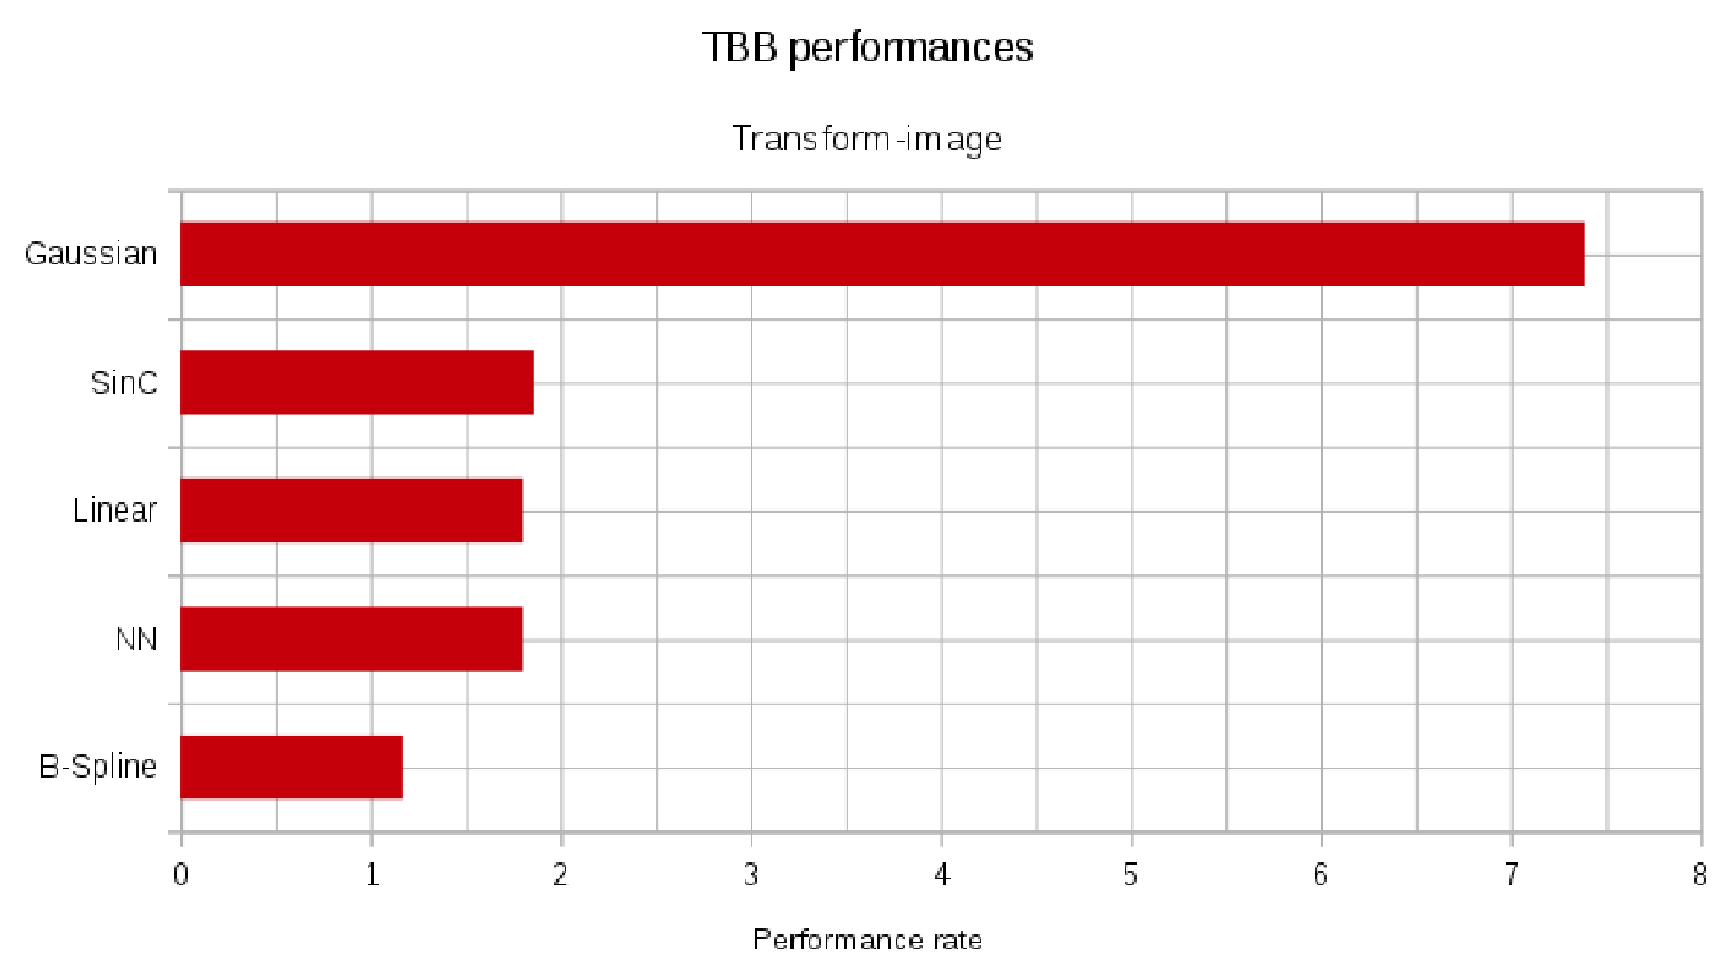
\includegraphics[width=10cm]{Reports/figures/performances_tbb_transform_image.eps}
		\caption{Améliorations apportées par TBB pour transform-image}
		\label{Améliorations apportées par TBB pour transform-image}
		\vspace{0.1cm}
	\end{subfigure}
	\begin{subfigure}{.5\textwidth}
		\centering
		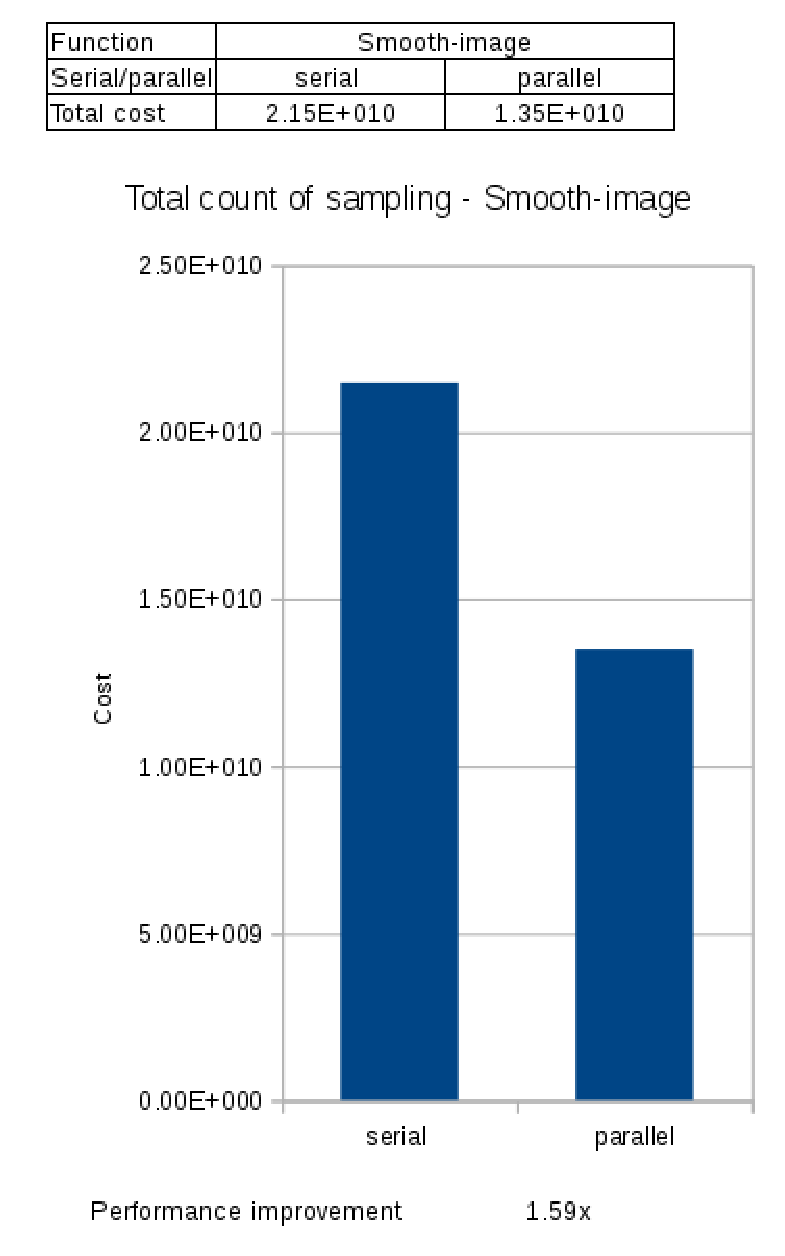
\includegraphics[width=6cm]{Reports/figures/smooth_image_costs.eps}
		\caption{Coût de la fonction de flou gaussien}
		\label{Coût de la fonction de flou gaussien}
	\end{subfigure}
	\caption{Relevés du nombre d'instructions}
	\label{Relevés du nombre d'instructions}
\end{figure}

A l'aide du module CacheGrind, il a été aussi possible de relever les fuites de caches et les mauvaises prédictions de branche:

\begin{figure}[h!]
	\begin{center}
		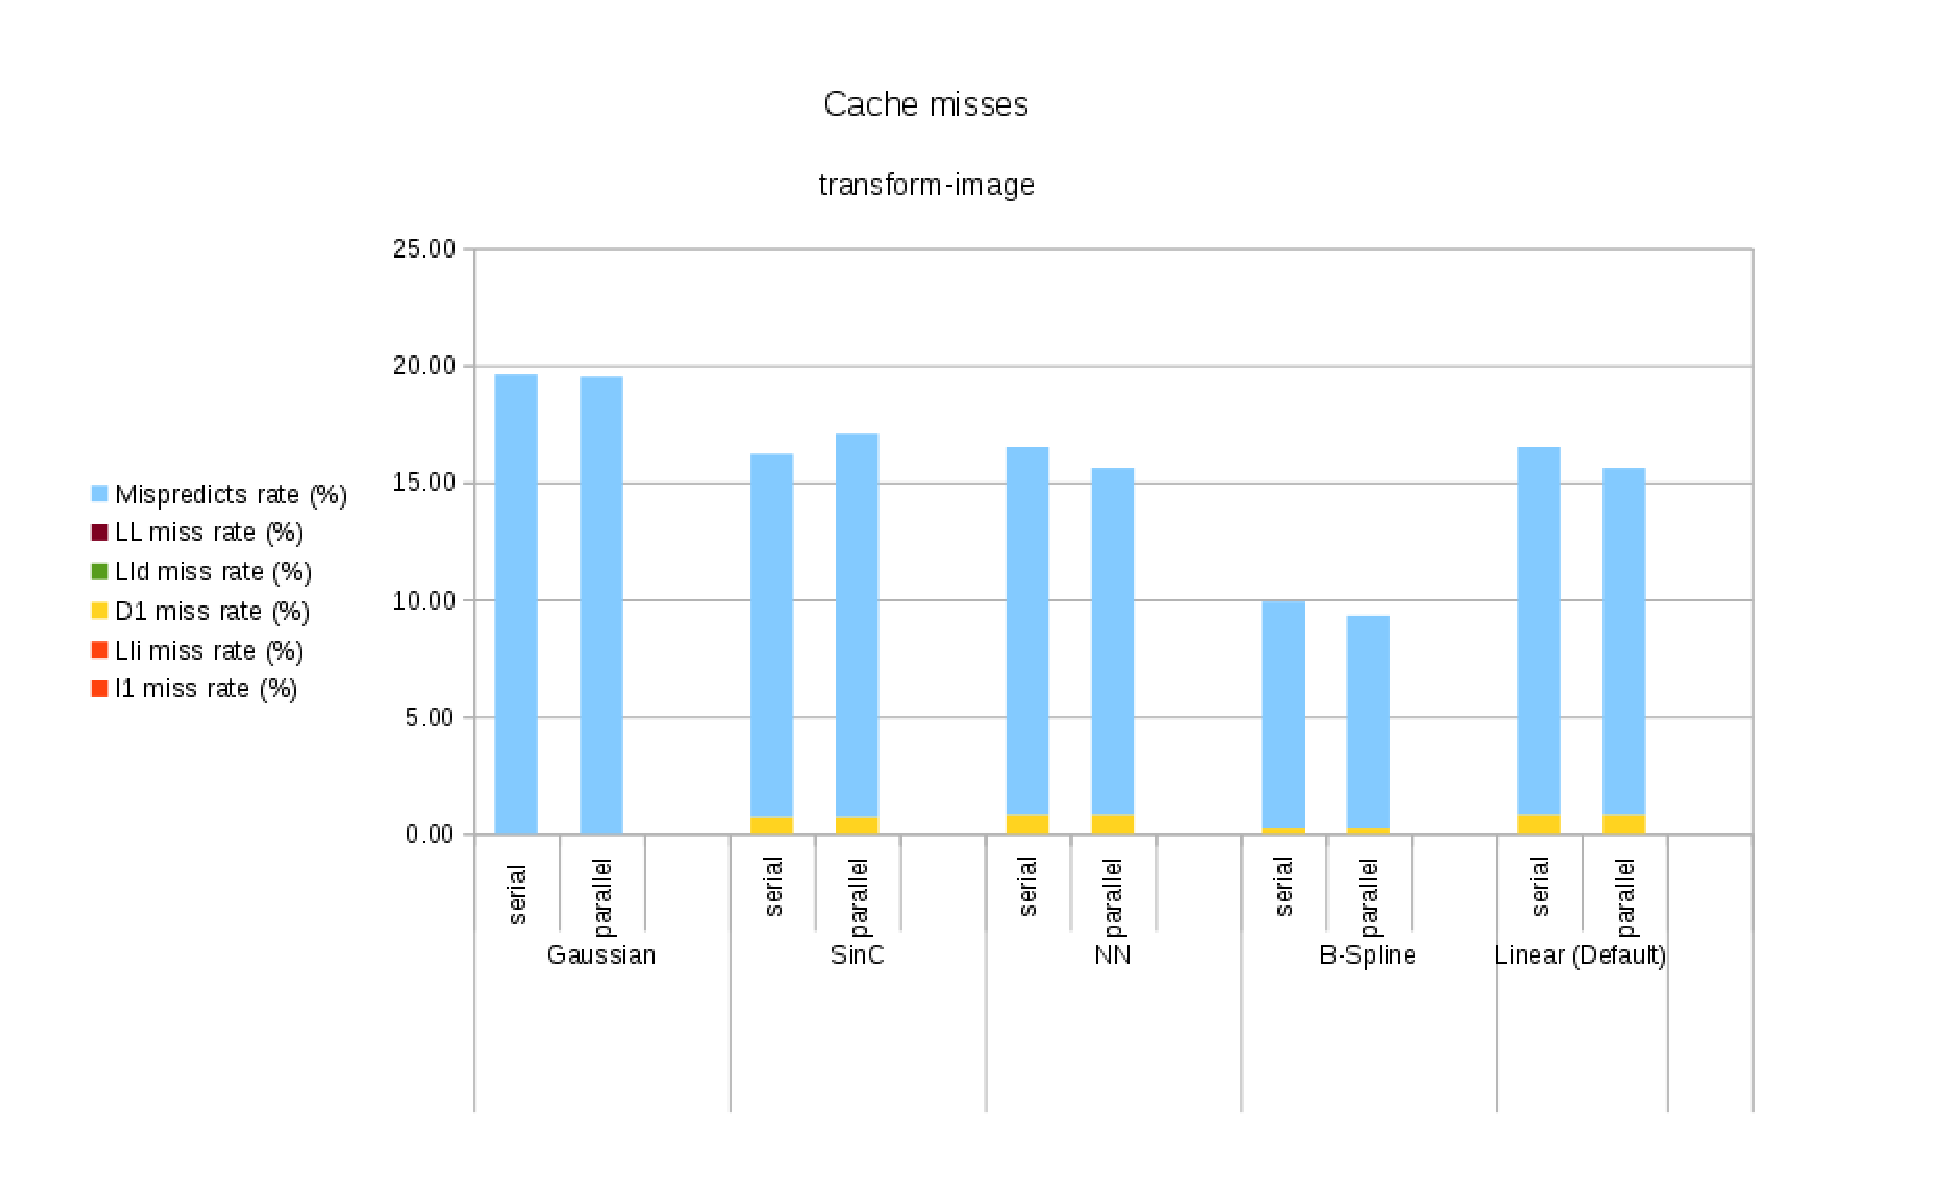
\includegraphics[width=15cm]{Reports/figures/cache_misses_transform_image.eps}
	\end{center}	
	\caption{Fuites de cache pour la fonction transform-image}
	\label{Fuites de cache pour la fonction transform-image}
\end{figure}~\par
Pour "transform-image", CacheGrind indique relativement peu de fuites de caches, mais, en revanche, le taux de mauvaise prédiction de branche vaut entre 10\% et 20\% en fonction de l'interpolation choisie. De plus, le taux de variation des mauvaises prédictions de branches et de fuites de caches est très faibles entre un code sérialisé et un code parallélisé avec les fonctionnalités présentes dans le MIRTK.\\
Les résultats concernant les fuites de cache pour transform-image sont très semblables pour smooth-image.
\subsection{Analyse}
    \paragraph{Analyse du nombre d'instructions}~\par
Callgrind étudie le coût, en nombre d'instructions CPU, des fonctions du programme profilé. Chaque instruction ayant le même temps d'exécution, le nombre d'instructions est proportionnel au temps. L'évolution relative du nombre d'instructions est donc équivalente à celle du temps d'exécution.\\
Pour transform-image, la parallélisation du code des différentes interpolation est inégale. L'interpolation gaussienne est quasiment parfaitement parallélisée, ce qui n'est pas le cas des autres interpolations de \textit{transform-image}. En effet, la machine possédant 8 coeurs, la parallélisation optimale serait à un taux x8, ce qui est le cas pour l'interpolation gaussienne seulement.\\
Concernant la fonction smooth-image, l'amélioration apportée par TBB est aussi faible, de l'ordre d'un taux de x1.59. La marge de réduction du temps d'exécution était encore grande.
\newpage
\paragraph{Analyse des fuites de cache}~\par
Cachegrind est un module qui simule l'interaction du programme avec la hiérarchie des caches. Les caches représentent une partie de la mémoire informatique, et enregistrent temporairement des copies de données provenant d'une source, afin de diminuer le temps d'un nouvel accès d'un CPU à ces données. Comme représenté en figure \ref{Différents niveaux de mémoire d'un microprocesseur}, il y a plusieurs niveaux de mémoire entre un CPU et sa mémoire principale. 

Sur la figure \ref{Différents niveaux de mémoire d'un microprocesseur} sont représenté 2 niveaux de mémoire cache, mais il est possible d'avoir plus ou moins de niveaux.
Les différents niveaux de mémoire cache sont désignés de la manière suivante : Level 1 (abrégé L1), Level 2 (abrégé L2) ... et le dernier niveau : Last Level (abrégé LL). Les niveaux de cache les plus bas correspondent aux caches les plus proches du CPU. 
\begin{figure}[h!]
	\begin{center}
		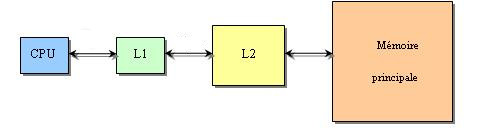
\includegraphics[width=13cm]{Reports/figures/Mem_hierarchy.jpg}
	\end{center}	
	\caption{Différents niveaux de mémoire d'un microprocesseur}
	\label{Différents niveaux de mémoire d'un microprocesseur}
\end{figure}~\par 
En plus des fuites de caches, CacheGrind est capable de relever d'autres informations pertinentes telles que les erreurs de prédiction de branchement.\\
La prédiction de branchement est une fonctionnalité d'un processeur qui lui permet de prédire le résultat d'un branchement. Avec cette technique, le processeur va faire de l’exécution spéculative : il va prédire le résultat d'un branchement, et va poursuivre l’exécution du programme avec le résultat de la prédiction. Si la prédiction échoue, les instructions chargées par erreur sont annulées. Dans ce cas-ci, CacheGrind relèvera une mauvaise prédiction de branche et engendrer des ralentissements possibles.\\
Dans le cas des fonctions profilées, les fuites de caches sont minimes, inférieures à 2 \%. En revanche, les erreurs de prédictions de branche sont de l'ordre de 20\%, ce qui reste suffisamment acceptable pour se focaliser sur le temps d'exécution uniquement.  
\newpage
\section{Diagramme de GANTT}
	\begin{figure}[h!]
		\begin{center}
			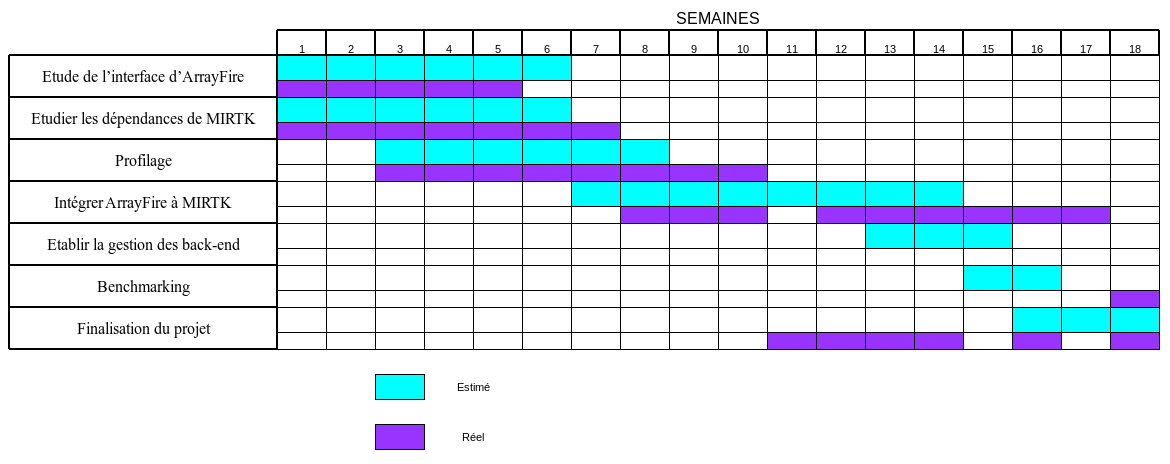
\includegraphics[width=18cm]{ganttchart.png}
		\end{center}	
		\caption{Diagramme de GANTT du stage}
		\label{Diagramme de GANTT du stage}
	\end{figure}
	Durant la première partie du stage, il était convenable de combiner de manière parallèle l'étude de l'interface d'ArrayFire et l'étude du MIRTK. De cette manière, j'ai pu corréler les fonctions utiles dans le MIRTK et les outils semblables disposés par ArrayFire.\\
	Le profilage a ensuite été le lien entre la phase d'étude et celle d'implémentation. \\
	Par manque de temps, la gestion optimisée des backends n'a pas été abordée, afin de finaliser le stage convenablement et d'obtenir tout de même quelques relevés de performances.
	
\chapter{Améliorations et perspectives} \vspace{-1cm}
Cette dernière partie du rapport détaille les travaux possibles suite à ce stage. Les perspectives à court et long terme sont détaillées séparément.

	\section{A cours terme}
	 La réduction du temps d'exécution des fonctions de transformation et de floutage devrait améliorer le temps d'exécution du recalage. Une fois le stage achevé sur le plan technique, il sera alors pertinent de vérifier l'amélioration des performances du module de recalage du MIRTK. Pour cela, il faudra procéder à un profilage de la fonction de recalage, idéalement sur différentes machines, et en faisant varier les paramètres d'entrée.\\
	 ArrayFire étant implanté que succinctement dans le MIRTK, il faudra porter son intégration sur les autres fonctionnalités du module mathématique du MIRTK, ainsi que sur les autres modules liés au recalage d'image.\\
	 Après ces différentes modifications et ajouts, il est possible que plusieurs fonctions seront dépréciées ou ré-implémentées, c'est pourquoi un réusinage* de l'intégralité du code source devra être entrepris, pour maintenir une certaine clarté dans le code source.\\ 

	\section{A long terme}
	Le MIRTK est un logiciel dont les fonctions et structures de données du MIRTK ont été conçues pour du traitement séquentiel, c'est-a-dire voxel par voxel. Modifier le code pour tirer avantage de l'accélération fournie par le calcul vectorisé est, par conséquent, plus difficile.\\
	Depuis quelques années, le code source du MIRTK à renforcé son interdépendance entre ses classes. De son architecture ressort maintenant un couplage "serré", qui, par opposition à un couplage "libre", reflète un agencement de classes très complexe, et qui reste déprécié. En plus de l'architecture séquentielle du traitement, ce couplage important restreint l'usinage du code du MIRTK.\\
	Le code source du MIRTK dérive de celui d'un logiciel plus ancien, appelé IRTK (Image Registration ToolKit). Cependant, peu d'améliorations techniques y ont été ajouté lors de sa refonte en MIRTK. C'est-à-dire que le langage employé, le C++, a été conservé, ou encore que les classes et structures de données ont été simplement étoffées de nouveaux attributs et méthodes. Le manque de direction dans le développement depuis plus de 15 ans induit aussi un manque de cohérence dans l'implémentation de ses différentes fonctionnalités. Par exemple, bien qu'il soit codé en C++, tous les modules n'utilisent pas systématiquement l'encapsulation offerte par le module mathématique pour l'implémentation de leurs algorithmes de calcul.\\	
	Puisque le MIRTK possède aujourd'hui un ensemble de structures de données centrées sur une exécution séquentielle, il faudra, à long terme modifier cette architecture pour l'orienter sur une exécution vectorisée en intégrant ArrayFire directement dans ce jeu de classes et de structures de données.\\ 
	Afin d'exploiter le potentiel d'un cluster GPU, il faudra enfin adapter l'exécution du MIRTK à un support multi-GPU.  

\chapter*{Conclusion} 
\addcontentsline{toc}{chapter}{Conclusion}
Afin de répondre au mieux à la problématique du stage, un profilage du MIRTK a tout d'abord permis de mettre en valeur les fonctions les plus intéressantes à améliorer: le floutage et la transformation homogène. Ces fonctions intervenant dans le cadre d'un recalage d'images, spécialité du MIRTK, elles ont été ré-implémentées en utilisant la bibliothèque mathématique performante ArrayFire. Outre ses capacités de vectorisation, ArrayFire permet aussi la gestion de différents backends, rendant l'exécution sur carte graphique totalement transparente. ArrayFire a ainsi permis de rester aisément dans le cadre du cahier des charges imposé en début de stage. Par la suite, ces travaux pourront être poussés davantage pour que le MIRTK soit intégré dans le projet d'UK BioBank.\\ ~\par
\noindent
Sur un plan personnel, j'ai pu tiré beaucoup de notions techniques de ce stage, en utilisant les outils d'un chercheur en informatique, tels que l'utilisation d'un logiciel de contrôle de version (GIT) ou l'apprentissage du langage LaTeX pour l'écriture de mes rapports. Par ailleurs, j'ai aussi pu appréhender le fonctionnement de base d'un logiciel de traitement d'images tel que le MIRTK, préparant de manière concrète ma cinquième année en option SA3I à l'INSA, tout en évoluant dans un milieu de recherche, qui m'était inconnu auparavant.
\chapter*{Sources}
\addcontentsline{toc}{chapter}{Sources}
\noindent
\url{https://biomedia.doc.ic.ac.uk/}  : site officiel du laboratoire BioMedIA. \\
\\
\url{http://www.imperial.ac.uk} : site officiel de l'Imperial Colleg London.\\
\\
\url{https://fr.wikipedia.org/wiki/Imperial_College_London} : article Wikipédia de l'Imperial College London.\\
\\
\url{http://www.ukbiobank.ac.uk/about-biobank-uk/} : article du site de UK BioBank présentant le projet.\\
\\
\url{http://ric.uthscsa.edu/mango/papaya/index.html} : outil de visualisation d'images en format NIFTI.\\
\\
\url{https://wiki.imperial.ac.uk/display/HPC/Systems} : données et statistiques de la grille de calcul de l'Imperial College.\\
\\
\url{http://www.egi.eu/} : site officiel de la grille européenne de calcul.\\
\\
\url{https://fr.wikipedia.org/wiki/Parall\%C3\%A9lisme_\%28informatique\%29}: article Wikipédia du parallélisme informatique.\\
\\
\url{https://fr.wikipedia.org/wiki/R\%C3\%A9usinage_de_code} : article Wikipédia du réusinage d'un code. \\
\\
\url{http://www.nvidia.fr/object/gpu-computing-fr.html}: article du site nvidia présentant le principe de fonctionnement d'une carte graphique.\\
\\
\url{https://fr.wikipedia.org/wiki/Recalage_d'images}: article Wikipédia du recalage d'images.\\
\\
\url{https://fr.wikipedia.org/wiki/Environnement_d'ex\%C3\%A9cution}: article Wikipédia de l'environnement d'exécution.\\
\\

\renewcommand{\listfigurename}{Table des illustations}\listoffigures 
\addcontentsline{toc}{chapter}{Table des illustrations}
\chapter*{Glossaire}
\addcontentsline{toc}{chapter}{Glossaire}
\noindent 

\textbf{\\CPU:} \textit{Central Processing Unit}, processeur. \vspace{2cm}
\textbf{\\Environnement d'exécution:}  logiciel responsable de l'exécution des programmes informatiques écrits dans un langage de programmation donné. Un environnement d'exécution offre des services d'exécution de programmes tels que les entrées-sorties, l'arrêt des processus, l'utilisation des services du système d'exploitation, le traitement des erreurs de calcul, la génération d'événements, l'utilisation de services offerts dans un autre langage de programmation, le débogage, le profilage et le ramasse-miette.\vspace{2cm} 
\textbf{\\GPU:} \textit{Graphics Processing Unit}, carte graphique.  \vspace{2cm}

\textbf{\\Réusinage d'un code (ou \textit{code refactoring}, en anglais):} opération consistant à retravailler le code source d'un programme informatique (sans toutefois y ajouter des fonctionnalités ni en corriger les bogues) de façon à en améliorer la lisibilité et par voie de conséquence la maintenance, ou à le rendre plus générique (afin par exemple de faciliter le passage de simple en multiple précision); on parle aussi de « remaniement ».  \vspace{2cm} 
\textbf{\\Thread:} entité d'exécution, c'est-à-dire une partie code qui peut être exécutée en un bloc. Le \textbf{multi-threading} est une méthode exécutant des blocs de code sur plusieurs threads.\vspace{2cm}
\textbf{\\Voxel:} équivalent d'un pixel, en 3 dimensions. Il s'agit d'une portion spatiale atomique d'une image qui représente une couleur unique, indiquée, dans le cadre du stage, par une valeur entre 0 et 255 (0 signifiant noir, et 255 blanc). Une haute résolution implique un nombre important de voxels et vice-versa.  
\definecolor{mygreen}{rgb}{0,0.6,0}
\definecolor{mygray}{rgb}{0.5,0.5,0.5}
\definecolor{mymauve}{rgb}{0.58,0,0.82}

\lstset{ %
	backgroundcolor=\color{white},   % choose the background color
	basicstyle=\footnotesize,        % size of fonts used for the code
	breaklines=true,                 % automatic line breaking only at whitespace
	captionpos=b,                    % sets the caption-position to bottom
	commentstyle=\color{mygreen},    % comment style
	escapeinside={\%*}{*)},          % if you want to add LaTeX within your code
	keywordstyle=\color{blue},       % keyword style
	stringstyle=\color{mymauve},     % string literal style
}

\begin{appendix}
	\chapter*{Annexe 1: Implémentation d'une fonction de recherche de valeurs propres en C++}
	\addcontentsline{toc}{chapter}{Annexe 1: Implémentation d'une fonction de recherche de valeurs propres en C++}
\vspace{-1cm}
\begin{lstlisting}[language=C++]
#include <arrayfire.h>
#include <cstdio>
#include <cstdlib>
// A preliminary test has been done to check whether the matrix is square and symmteric or not
af::array EigenValuesSolver(af::array &in) // the input is an array
{
	int size = in.dims(0); // gets dimensions of the input array
	int coltemp = 0;
	int rowtemp = 0;
	unsigned index = 0;
	float maxi = 0;
	float last_value;
	float new_value;
	float threshold = 0.001; // sets a threshhold for the stopping condition of the algorithm
	af::array U = af::identity(size, size);
	af::array V;
	af::array A = in; // copy the input array into a local variable
	af::array alpha = af::constant(1, 1, 1); // stores a numeric variable in an array
	af::array temp;
	
	/* Starts a Jacobi algorithm */
	do
	{
		last_value = maxi; // keeps the previous maximum value of A 
		
		/* Gets the maximum value from A outside its diagonal */
		temp = af::abs(A-af::diag(af::diag(A), 0, false)); 
		af::max(&maxi, &index, temp);  
		rowtemp = index%size;         // gets maximum value's row index
		coltemp = index/size;         // gets maximum value's column index
		
		/* Calculates the new rotation angle */
		alpha = 0.5*atan(2*A(rowtemp, coltemp)/(A(coltemp, coltemp)-A(rowtemp, rowtemp)));
		
		/* Creates the new rotation matrix */
		V = af::identity(size, size);
		V(rowtemp, coltemp) = sin(alpha);
		V(coltemp, coltemp) = cos(alpha);
		V(rowtemp, rowtemp) = cos(alpha);
		V(coltemp, rowtemp) = -sin(alpha);
		
		/* Final multiplications */
		A = af::matmul((af::transpose(V)),A,V); 
		U = af::matmul(U,V);
		
		new_value = maxi; // update the maximum value 
	}while(abs(last_value-new_value) > threshold); // loop condition
	
	return af::diag(A); // eigen values of the input are returned by getting
}

\end{lstlisting}

\chapter*{Annexe 2: Implémentation de "smooth-image" en Python}
\addcontentsline{toc}{chapter}{Annexe 2: Implémentation de "smooth-image" en Python}
\vspace{-1cm}
\begin{lstlisting}[language=python]
import arrayfire as af
import matplotlib.pyplot as plt
import nibabel as nib 
from scipy import signal
import numpy as np
import argparse as ap
	
# Command line arguments and options handling 
parser = ap.ArgumentParser()
parser.add_argument("InputImage", type=str, help="Path to the input image")
parser.add_argument("OutputImage", type=str, help="Path to the input image")
parser.add_argument("Sigma", type=int, help="Defines the value of sigma for the Gaussian kernel. Default: 1")
parser.add_argument("--dimension", type=str, choices=["x", "y", "z", "xy", "yz", "xz", "xyz"], help="Specifies on which dimensions execute the blurring. Default: xyz")
parser.add_argument("-color", help="Enable colored input/output image plot.", action="store_false")
parser.add_argument("-nodisplay", help="Cancel plot of the input/output images. Has priority over \"-color argument\".", action="store_false")

args = parser.parse_args()

# Loading input
img = nib.load(args.InputImage)
hdr = img.get_header()
img_data = img.get_data().astype('f')

# Conversion numpy => arrayfire
img_data_af = af.interop.np_to_af_array(img_data)

# Declaration of Gaussian kernel
if args.Sigma:
	kernel = signal.gaussian(img_data.shape[0], std = args.Sigma).astype('f')
else:
	kernel = signal.gaussian(img_data.shape[0], std = 1).astype('f')

# Conversion numpy => arrayfire for the Gaussian kernel
kernel_af = af.interop.np_to_af_array(kernel)

# Convolution along dimensions chosen 
output_image = img_data_af.copy()
input_image = img_data_af.copy()

if (args.dimension):

	if ("x" in args.dimension):
		output = af.convolve1(input_image, kernel_af)
	
	if ("y" in args.dimension):
		input_image = af.reorder(output_image, 1, 0, 2)
		output_image = af.convolve1(input_image, kernel_af)
		output_image = af.reorder(output_image, 1, 0, 2)
	
	if ("z" in args.dimension):
		input_image = af.reorder(output_image, 2, 1, 0)
		output_image = af.convolve1(input_image, kernel_af)
		output_image = af.reorder(output_image, 2, 1, 0)
else:
	output_image = af.convolve1(input_image, kernel_af)
	input_image = af.reorder(output_image, 1, 0, 2)
	output_image = af.convolve1(input_image, kernel_af)
	output_image = af.reorder(output_image, 1, 0, 2)
	input_image = af.reorder(output_image, 2, 1, 0)
	output_image = af.convolve1(input_image, kernel_af)
	output_image = af.reorder(output_image, 2, 1, 0)


# Conversion arrayfire => numpy
output_np = output_image.to_array()
output_np = np.asarray(output_np)
output_np = output_np.reshape(320, 250, 202, order='F')

# Saving the output file
affine = img.get_affine()
new_img = nib.Nifti1Image(output_np, affine)
nib.save(new_img, args.OutputImage)

# Check if plot is not cancelled by "-nosdisplay" argument
if (args.nodisplay == True):
	# Assimilating color option
	if (args.color):
		colors = 'gray'
	else:
		colors = None
	
	# Ploting 1rst window
	f,fig = plt.subplots(1, 2)
	fig[0].imshow(img_data[125, :, :].T, extent=[0, hdr['pixdim'][1], 0, hdr['pixdim'][3]], cmap=colors, origin='lower')
	fig[1].imshow(output_np[125, :, :].T, extent=[0, hdr['pixdim'][1], 0, hdr['pixdim'][3]], cmap=colors, origin='lower')
	plt.suptitle("Gaussian Blurring on x-axis")
	
	# Ploting 2nd window
	f2,fig2 = plt.subplots(1, 2)
	fig2[0].imshow(img_data[:, 125, :].T, extent=[0, hdr['pixdim'][1], 0, hdr['pixdim'][3]], cmap=colors, origin='lower')
	fig2[1].imshow(output_np[:, 125, :].T, extent=[0, hdr['pixdim'][1], 0, hdr['pixdim'][3]], cmap=colors, origin='lower')
	plt.suptitle("Gaussian Blurring on y-axis")
	
	# Ploting 3rd window
	f3,fig3 = plt.subplots(1, 2)
	fig3[0].imshow(img_data[:, :, 125].T, cmap=colors, origin='lower')
	fig3[1].imshow(output_np[:, :, 125].T, cmap=colors, origin='lower')
	plt.suptitle("Gaussian Blurring on z-axis")
	
	plt.show()
	\end{lstlisting}

\end{appendix}

\end{document}
